%%%%%%%%%%%%%%%%%%%%%%%%%%%%%%%%%%%%%%%%%%%%%%
% 1. Document Class

\documentclass[a4paper,12pt]{report}
\renewcommand{\familydefault}{\sfdefault} % tipo de letra general

%%%%%%%%%%%%%%%%%%%%%%%%%%%%%%%%%%%%%%%%%%%%%%
% 2. Paquetes
%\PassOptionsToPackage{table}{xcolor}
\usepackage[utf8]{inputenc}
\usepackage[english]{babel}
\usepackage[top = 2.5cm, bottom = 2.5cm, left = 2.5cm, right = 2.5cm]{geometry}
\usepackage{ae,aecompl,amsmath,amsfonts,amssymb,graphicx}
\usepackage{wrapfig,float,titlesec,titletoc,fancyhdr,parskip}
\usepackage{mathrsfs,subfig,color,multicol,amscd,eso-pic}
\usepackage[usenames,dvipsnames,svgnames,table]{xcolor}
\usepackage[most]{tcolorbox}
\usepackage{subcaption}
\usepackage[T1]{fontenc}
\usepackage[colorlinks=true,linkcolor={RedOrange},citecolor={Purple},breaklinks=true,linktocpage]{hyperref}
%\spanishdecimal{.}
\usepackage{enumitem}
\usepackage{listings,transparent}
\lstset{language=Matlab}
\definecolor{codegreen}{rgb}{0,0.6,0}
\definecolor{codegray}{rgb}{0.5,0.5,0.5}
\definecolor{codepurple}{rgb}{0.44,0.0,0.1}
\definecolor{mediumblue}{rgb}{0.0,0.0,0.8}
%\definecolor{electricviolet}{rgb}{}
\definecolor{backcolour}{rgb}{0.95,0.95,0.92}
\lstdefinestyle{mystyle}{
	backgroundcolor=\color{backcolour},   
	commentstyle=\color{codegreen},
	keywordstyle=\color{blue},
	numberstyle=\tiny\color{codegray},
	stringstyle=\color{codepurple},
	basicstyle=\ttfamily\footnotesize,
	breakatwhitespace=false,         
	breaklines=true,                 
	captionpos=t,                    
	keepspaces=true,                 
	numbers=left,                    
	numbersep=6pt,                  
	showspaces=false,                
	showstringspaces=false,
	showtabs=false,                  
	tabsize=2 }
\lstset{style=mystyle}
\renewcommand\lstlistingname{\bf Código}
\renewcommand\lstlistlistingname{Códigos}

%%%%%%%%%%%%%%%%%%%%%%%%%%%%%%%%%%%%%%%%%%%%%%%
% Marca de agua
\AddToShipoutPicture{
	\put(0,0){
		\parbox[b][\paperheight]{\paperwidth}{
			\vfill
			\centering
			{\transparent{0.2}
\includegraphics[scale=0.8]{IMAGENES/logo}}
			\vfill
		}
	}
}

%%%%%%%%%%%%%%%%%%%%%%%%%%%%%%%%%%%%%%%%%%%%%%
% Estilo de paginas
\pagestyle{fancy}
%\renewcommand{\headrule}{\color{Orange} \titlerule}
\fancyhf{}
\lhead{\footnotesize \color{BrickRed} \large Cómputo Científico} % esquina izquierda
\rhead{\footnotesize \color{BrickRed} \large Tarea 5} % esquina derecha
\cfoot{\color{NavyBlue} \bfseries\thepage }

\title{Tarea 5}
\author{Ezau Torres}

%%%%%%%%%%%%%%%%%%%%%%%%%%%%%%%%%%%%%%%%%%%%%%
% DOCUMENTO

\begin{document}
	\begin{minipage}{0.15\textwidth}
		\centering
		
\includegraphics[width=\textwidth]{IMAGENES/logo}
	\end{minipage}
	\begin{minipage}{0.85\textwidth}
		\centering
		\textbf{\large Cómputo Científico para Probabilidad, Estadística y Ciencia de Datos}\\
		\medskip
		\text{\large Ezau Faridh Torres Torres} \\
		\medskip
		\textbf{\large TAREA 5: Simulación Estocástica, introducción.}\\
		\medskip
%		\text{Maestría en Ciencias Matemáticas Aplicadas}\\
%		\medskip
		\textbf{Fecha de entrega:} 09/Oct/2024.
	\end{minipage}

\vspace{5mm}

%%%%%%%%%%%%%%%%%%%%%%%%%%%%%%%%%%%%%%%%%%%%%%
% CONTENIDO
%%%%%%%%%%%%%%%%%%%%%%%%%%%%%%%%%%%%%%%%%%%%%%

\textcolor{BrickRed}{\bf NOTA:}  Los ejercicios se encuentran repartidos en los archivos:
\begin{itemize}
	\item \textcolor{mediumblue}{ejercicio2\_tarea5.py}
	\item \textcolor{mediumblue}{ARS.py}
	\item \textcolor{mediumblue}{ejercicio5\_tarea5.py}
\end{itemize}

% ------------------------------------------------------------------------------------
\vspace{5mm}
{\color{lightgray} \hrule}
\begin{enumerate}
	\item Sean $x_i \sim G a(\alpha, \beta)$; $i=1,2, \ldots, n$. Simular datos $x_i$ con $\alpha=3$ y $\beta=100$ considerando los casos $n=5$ y $40$.
	
	Con $\alpha \sim \mathrm{U}(1,4), \beta \sim \exp (1)$ distribuciones a priori, se tiene la posterior
	\begin{equation} \label{eq:1}
		 f(\alpha, \beta \mid \bar{x}) \propto \frac{\beta^{n \alpha}}{\Gamma(\alpha)^n} r_1^{\alpha-1} e^{-\beta\left(r_2+1\right)} \cdot \mathbbm{1}_{(1 \leq \alpha \leq 4)} \cdot \mathbbm{1}_{(\beta>1)}
	\end{equation}
	con
	\begin{equation} \label{eq:2}
		r_2= \sum_{i=1}^n x_i \text { y } r_1=\prod_{i=1}^n x_i
	\end{equation}
	
	En ambos casos, grafica los contornos para visualizar dónde está concentrada la posterior. Utilizar la propuesta
	\begin{equation} \label{eq:3}
		q\left(\left.\binom{\alpha_p}{\beta_p} \right\rvert\,\binom{\alpha}{\beta}\right)=\binom{\alpha}{\beta}+\binom{\varepsilon_1}{\varepsilon_2}
	\end{equation}
	donde
	\begin{equation}
		\binom{\varepsilon_1}{\varepsilon_2} \sim \mathcal{N}_2\left( \binom{0}{0}, \left(
		\begin{array}{cc}
			\sigma_1^2 & 0 \\
			0 & \sigma_2^2
		\end{array}
		\right)\right).
	\end{equation}
\end{enumerate}

\textcolor{BrickRed}{\it Respuesta:}

En el archivo \textcolor{mediumblue}{ejercicio1\_tarea7.py} se implementa la función \textit{METROPOLIS\_HASTINGS\_SIM()} la cual aplica el algoritmo Metropolis-Hastings para propuestas simétricas simulando una cadena de Markov en $\mathbb{R}^n$ y toma los siguientes argumentos:
\begin{itemize}
	\item La función objetivo $f$ (en este caso es la posterior \eqref{eq:1}).
	\item La distribución propuesta $q_{gen}$ (en este caso es la propuesta \eqref{eq:3}).
	\item El valor inicial $x_0$ (en este caso es $(\alpha, \beta)$ con $\alpha \sim \mathrm{U}(1,4), \beta \sim \exp (1)$).
	\item El número de iteraciones del algoritmo (casi siempre se usa $N = 10,000$).
\end{itemize}

Regresa la cadena de Markov simulada en $\mathbb{R}^n$ y usa el criterio de aceptación: si $y_t$ es la propuesta dada por $q_{gen}(\cdot|x_t)$ en $x_t$, entonces se acepta $y_t$ con probabilidad $\rho(x_t, y_t)$ con
\begin{equation}
	\rho(x,y) = \min\left\{1, \frac{f(y)}{f(x)} \right\}
\end{equation}
(en este caso, $\frac{q(x|y)}{q(y|x)} = 1$ ya que la propuesta es simétrica) y se rechaza con probabilidad $1-\rho(x_t, y_t)$. A continuación, se define la función \textit{SIMULAR\_GAMMA()}, la cual hace las simulaciones $x_i \sim G a(\alpha, \beta)$; $i=1,2, \ldots, n$

Después, se define la función posterior \eqref{eq:1} llamada \textit{posterior()}, y la función \textit{propuesta\_gen()} dada por \eqref{eq:3} la cual, como vimos en clase, es simétrica. Dentro de la función \textit{posterior()} se aplicó el logaritmo a los términos para evitar desbordamientos numéricos.

Finalmente:
\begin{itemize}
	\item Se simulacion $x_i \sim G a(\alpha = 3, \beta=100)$; $i=1,2, \ldots, n$ para los casos $n_{1}=5$ y $n_{2}=40$.
	\item Se dio el punto inicial $x_0=(\alpha_0, \beta_0)$ con $\alpha_0 \sim \mathrm{U}(1,4), \beta_0 \sim \exp (1)$. Tal punto resultó ser: $(3.886, 1.007)$.
	\item Se aplicó el algoritmo Metropolis-Hastings para generar las cadenas correspondientes para $n_1$ y $n_2$ usando $N=10,000$ iteraciones.
	\item Se usaron los parámetros de varianza de la propuesta $\sigma_1=0.1$ y $\sigma_2=10$ (se comenta más de esta elección al final).
	\item Se generaron los histogramas resultantes de $\alpha$ y $\beta$ para ambs casos y se graficaron los contornos para visualizar la concentración de la posterior.
\end{itemize}

Se obtuvieron los siguientes resultados: para $n_1=5$ se obtuvo una tasa de aceptación del $18.45\%$ y el promedio de la cadena para cada parámetro resultó ser: $(1.163, 6.006)$ Mientras que para $n_2=40$ se obtuvo una tasa de aceptación del $21.42\%$ y el promedio de la cadena para cada parámetro resultó ser: $(1.131, 19.920)$. Los histogramas resultantes se encuentran en la figura siguiente:
\begin{figure}[h]
	\centering
	\begin{minipage}{0.495\textwidth}
		\centering
		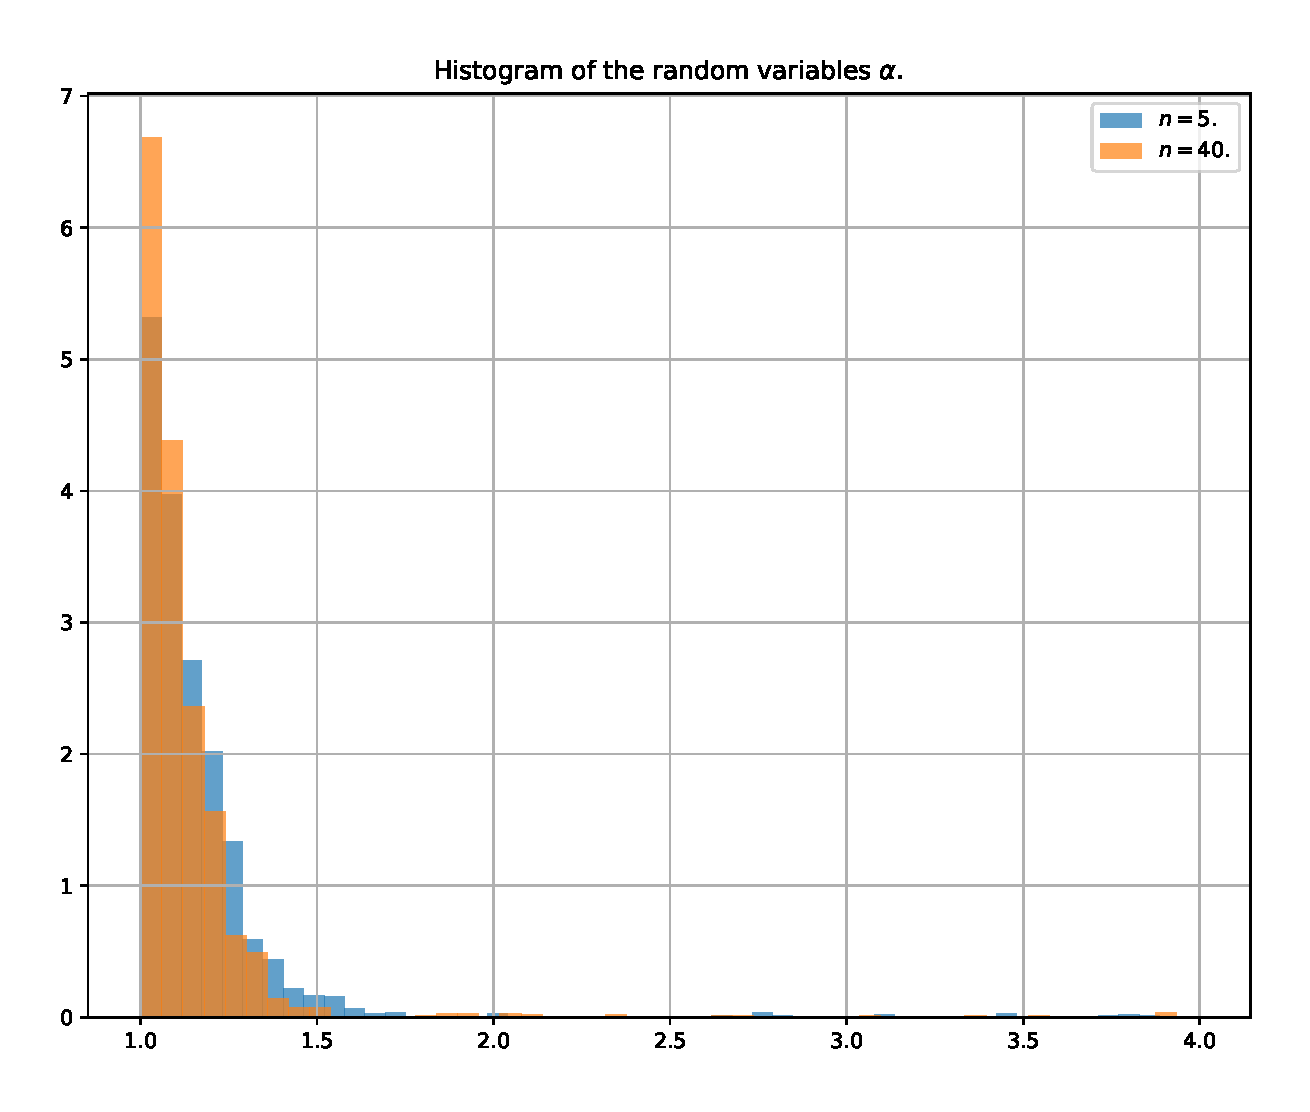
\includegraphics[width=\textwidth]{IMAGENES/ex1/histogram_n5.pdf}
		\caption{$\alpha$.}
	\end{minipage}
	\hfill
	\begin{minipage}{0.495\textwidth}
		\centering
		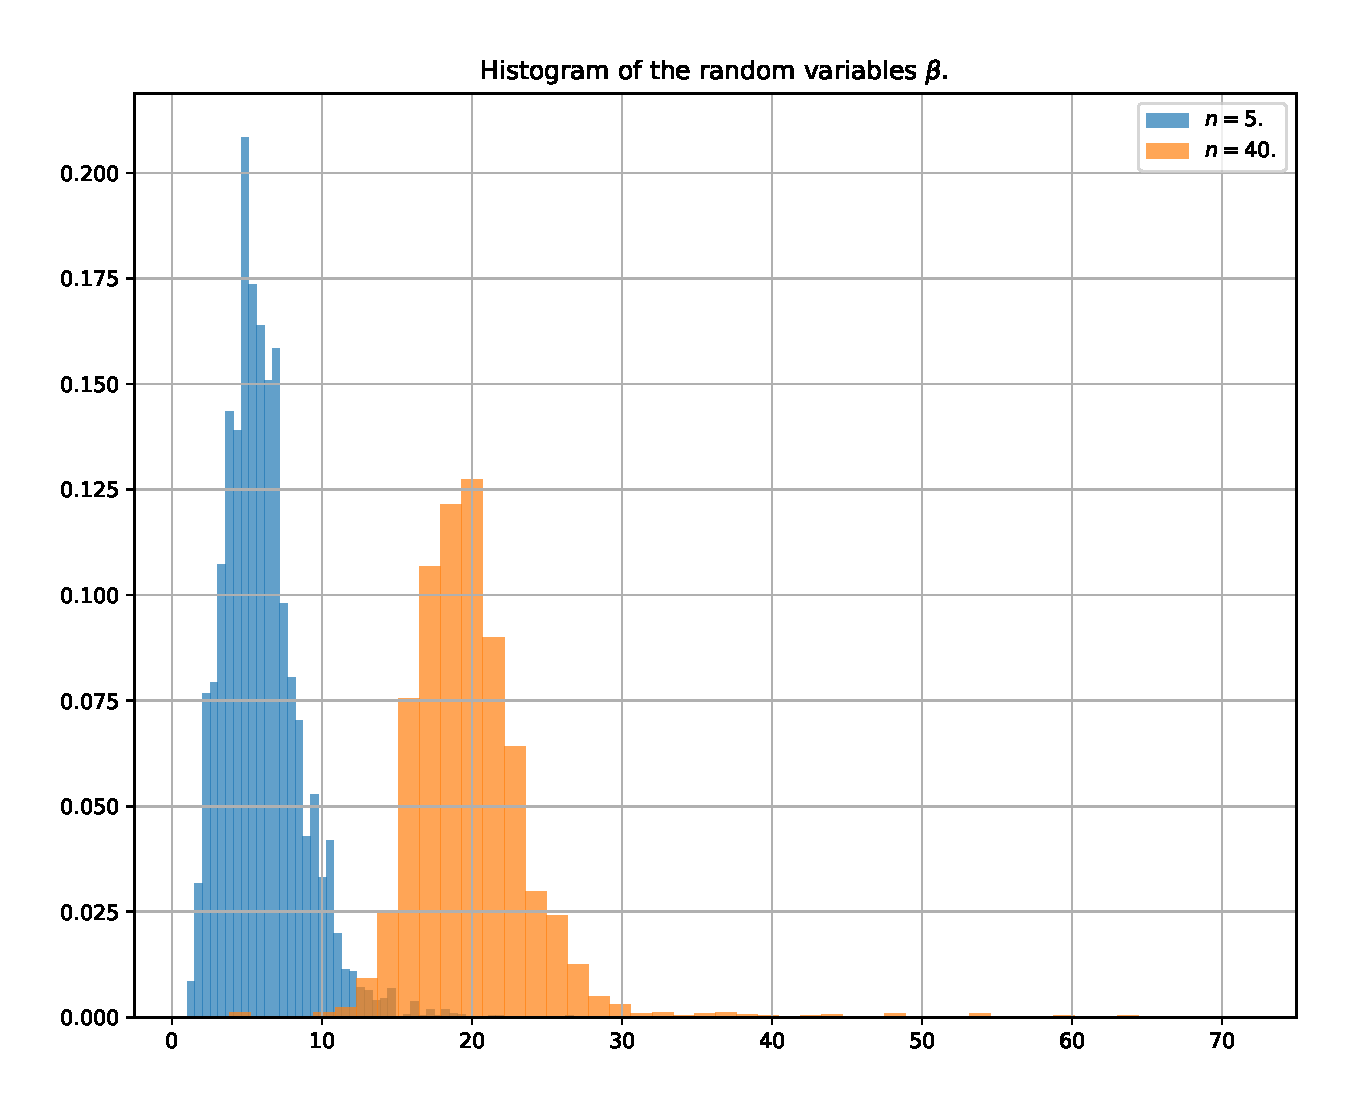
\includegraphics[width=\textwidth]{IMAGENES/ex1/histogram_n40.pdf}
		\caption{$\beta$.}
	\end{minipage}
\end{figure}

El gráfico de contornos es:
\begin{figure}[h!]
	\centering
	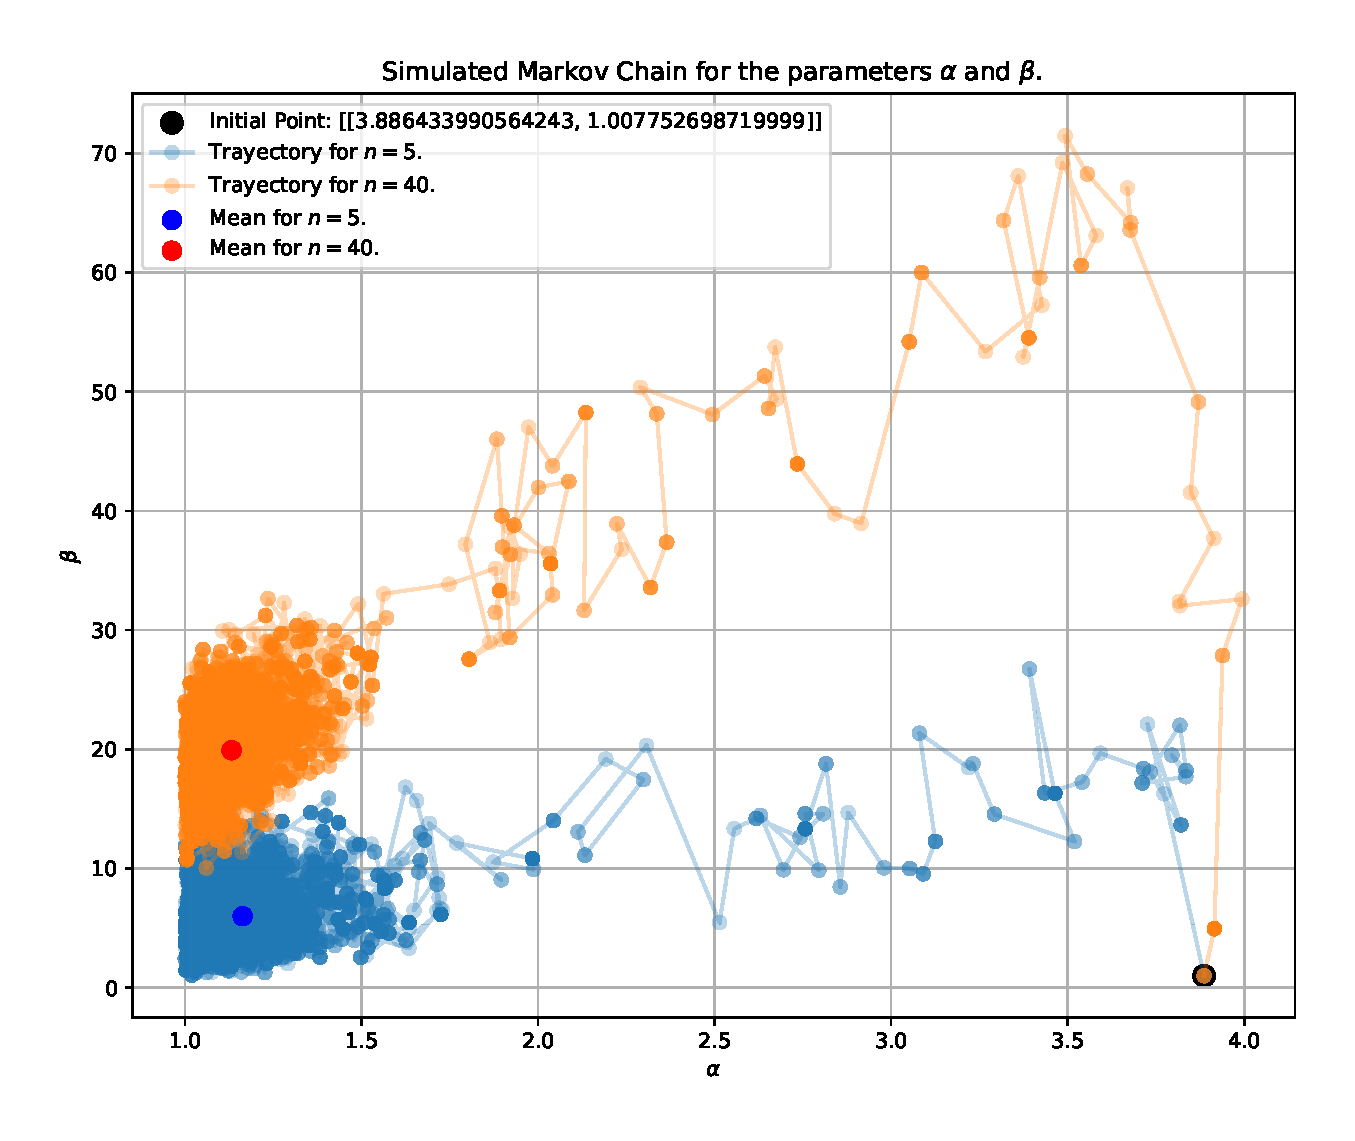
\includegraphics[width=0.76\textwidth]{IMAGENES/ex1/trayectory_ex1.pdf}
\end{figure}

Nótese que los valores promedio de las cadenas generadas se encuentran los puntos rojo y azul del gráfico anterior. En este caso particular, se puede ver que existe más varianza en el eje vertical, esto debido a que se tomó $\sigma_2$ $100$ veces mayor que $\sigma_1$. Otro ejemplo con varianzas distintas es:
\begin{figure}[h!]
	\centering
	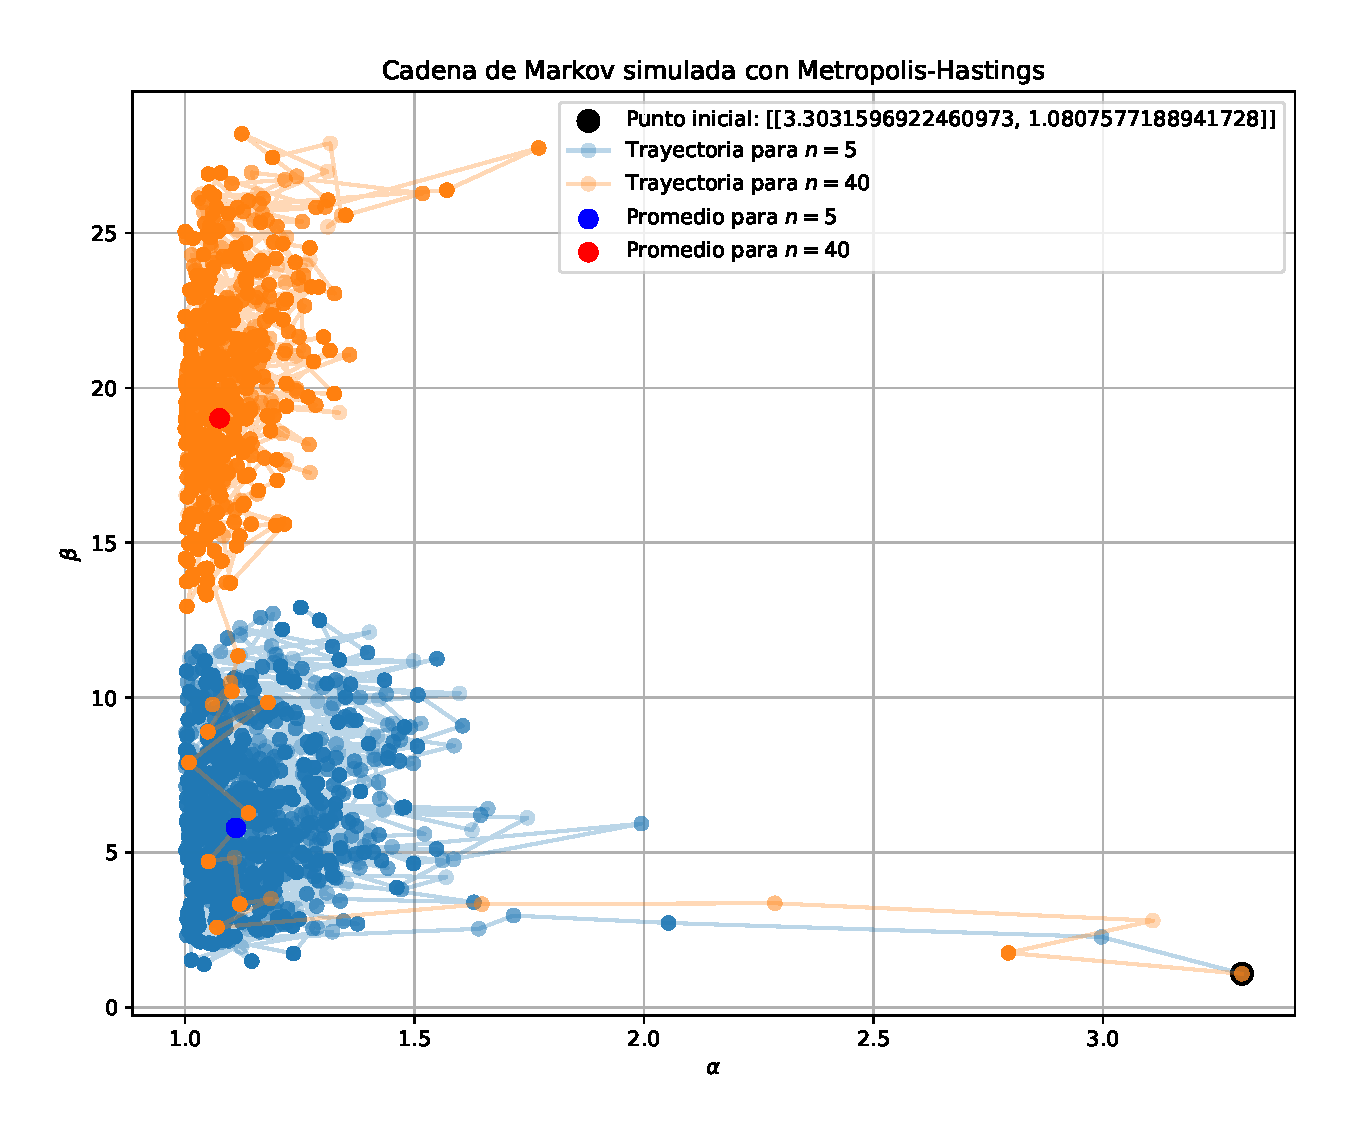
\includegraphics[width=0.76\textwidth]{IMAGENES/ejer12.pdf}
\end{figure}

En este último caso, se usó $\sigma_1=\sigma_2=1$. Sin importar el punto inicial, las varianzas elegidas o llevar el número de iteraciones a valores muy grandes, el algoritmo siempre terminaba alrededor de los mismos puntos, lo cual no corresponde con lo esperado ya que sabemos que los valores usados para generar las muestras fueron $\alpha=3$ y $\beta=100$. Incluso se varió $n$ para tener muestras más grandes y el resultado era similar (aunque sí hacía crecer los promedios de la cadena) o se volvía imposible de obtener debido a que el cálculo de $r_1$ causaba muchas indeterminaciones.
% ------------------------------------------------------------------------------------
\newpage
{\color{lightgray} \hrule}
\begin{enumerate} \setcounter{enumi}{1}
	\item Simular de la distribución $Gamma(\alpha,1)$ con la propuesta $Gamma([\alpha],1)$, donde $[\alpha]$ denota la parte entera de $\alpha$. Además, realizar el siguiente experimento: poner como punto inicial $x_0 = 950$ y graficar la evolución de la cadena, es decir, $f(X_t)$ vs $t$.
\end{enumerate}

\textcolor{BrickRed}{\it Respuesta:}

En el archivo \textcolor{mediumblue}{ejercicio2\_tarea7.py} se implementa la función \textit{METROPOLIS\_HASTINGS()} la cual aplica el algoritmo Metropolis-Hastings para cualquier dimensión $n$ y toma los siguientes argumentos:
\begin{itemize}
	\item La función objetivo $f$ (en este caso es una distribución $Gamma(\alpha,1)$).
	\item La distribución propuesta $q_{gen}$ (en este caso es una distribución $Gamma([\alpha],1)$).
	\item La función $q_{pdf}$ la cual es función de densidad de probabilidad de la propuesta $q_{gen}$.
	\item El valor inicial $x_0$ (en este caso es $x_{0}=950$).
	\item El número de iteraciones del algoritmo (casi siempre se usa $N = 10,000$).
\end{itemize}

Esta función regresa la cadena de Markov simulada. Usa el criterio de aceptación: si $y_t$ es la propuesta dada por $q(\cdot|x_t)$ en $x_t$, entonces se acepta $y_t$ con probabilidad $\rho(x_t, y_t)$ con
\begin{equation}
	\rho(x,y) = \min\left\{1, \frac{f(y)}{f(x)} \frac{q(x|y)}{q(y|x)} \right\}
\end{equation}
y se rechada con probabilidad $1-\rho(x_t, y_t)$ (para este caso se utiliza $q_{pdf}$).  Se define la función objetivo \textit{f()} (que es la pdf de una distribución $Gamma(\alpha,1)$), y las funciones propuesta \textit{q\_gen()} y \textit{q\_pdf()} dada por la distribución $Gamma([\alpha],1)$. Finalmente, se simulan variables aleatorias $Gamma(\alpha, 1)$ con $3$ alphas distintos y se comparan las distribuciones obtenidas con un histograma, también se genera el gráfico que describe la evolución de la cadena. Dado que $x_0=950$ es relativamente grande, $\alpha$ no tiene que ser tan alejado de $950$ para evitar indeterminaciones y el riesgo de no converger. Para esto, se tomaron los $3$ valores de $\alpha$ tales que:
\begin{itemize}
	\item $\alpha\in[x_0-200, x_0+200]$
\end{itemize}
\begin{figure}[h!]
	\centering
	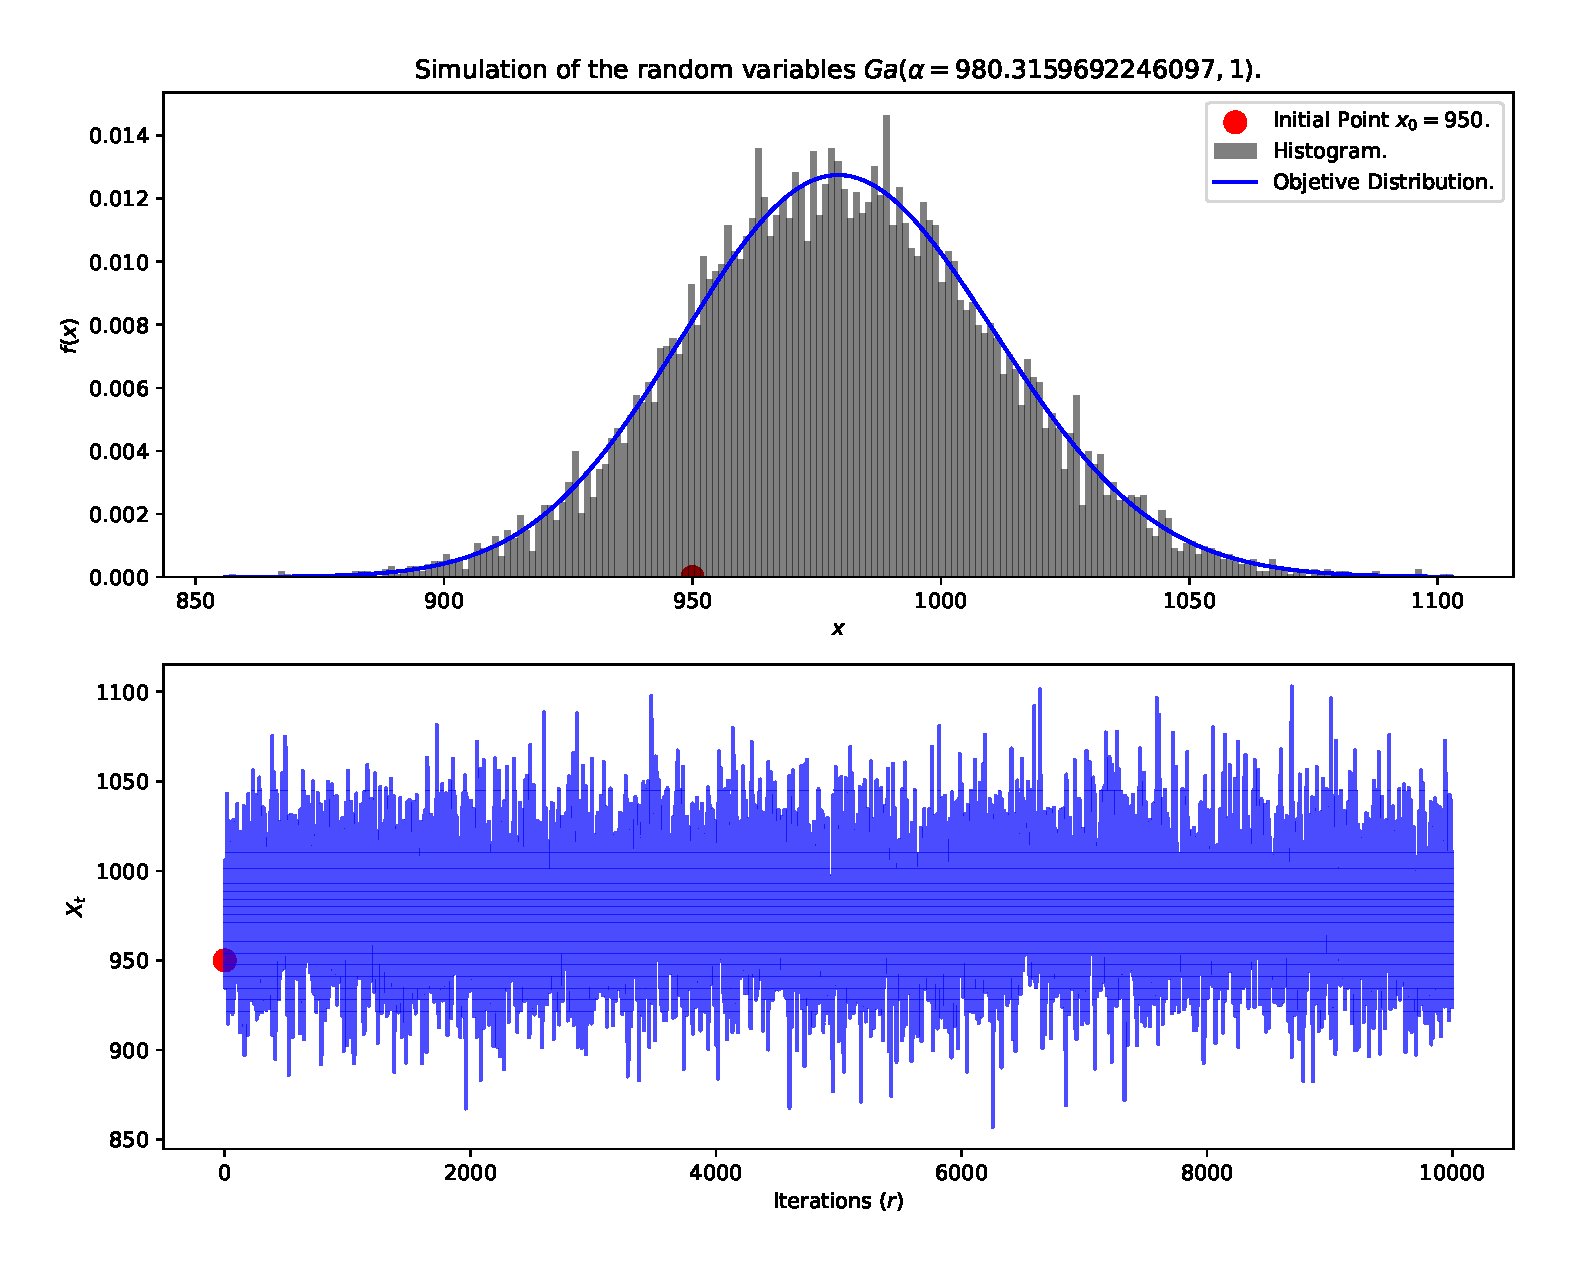
\includegraphics[width=0.6\textwidth]{IMAGENES/ex2/example1_ex2.pdf}
\end{figure}

\begin{itemize}
	\item $\alpha\in[x_0-500, x_0]$
\end{itemize}
\begin{figure}[h!]
	\centering
	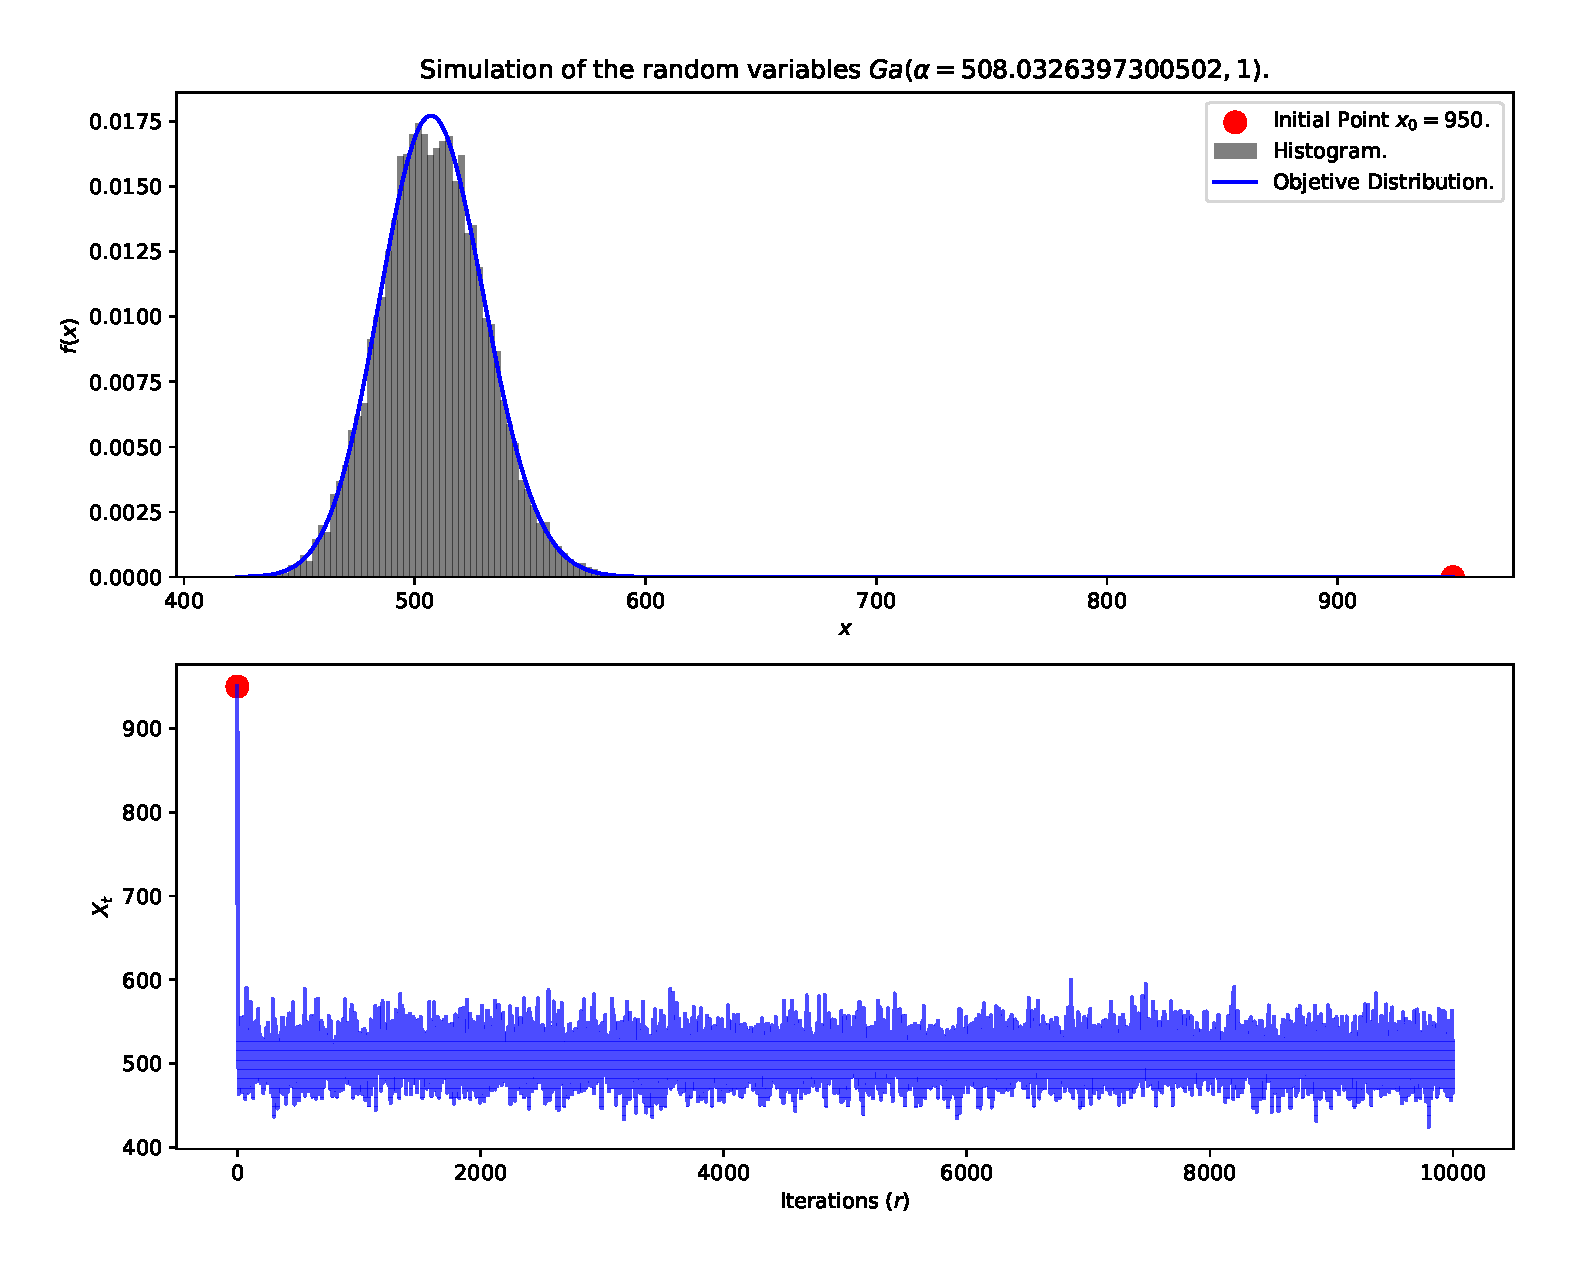
\includegraphics[width=0.6\textwidth]{IMAGENES/ex2/example2_ex2.pdf}
\end{figure}

\begin{itemize}
	\item $\alpha\in[x_0, x_0+500]$
\end{itemize}
\begin{figure}[h!]
	\centering
	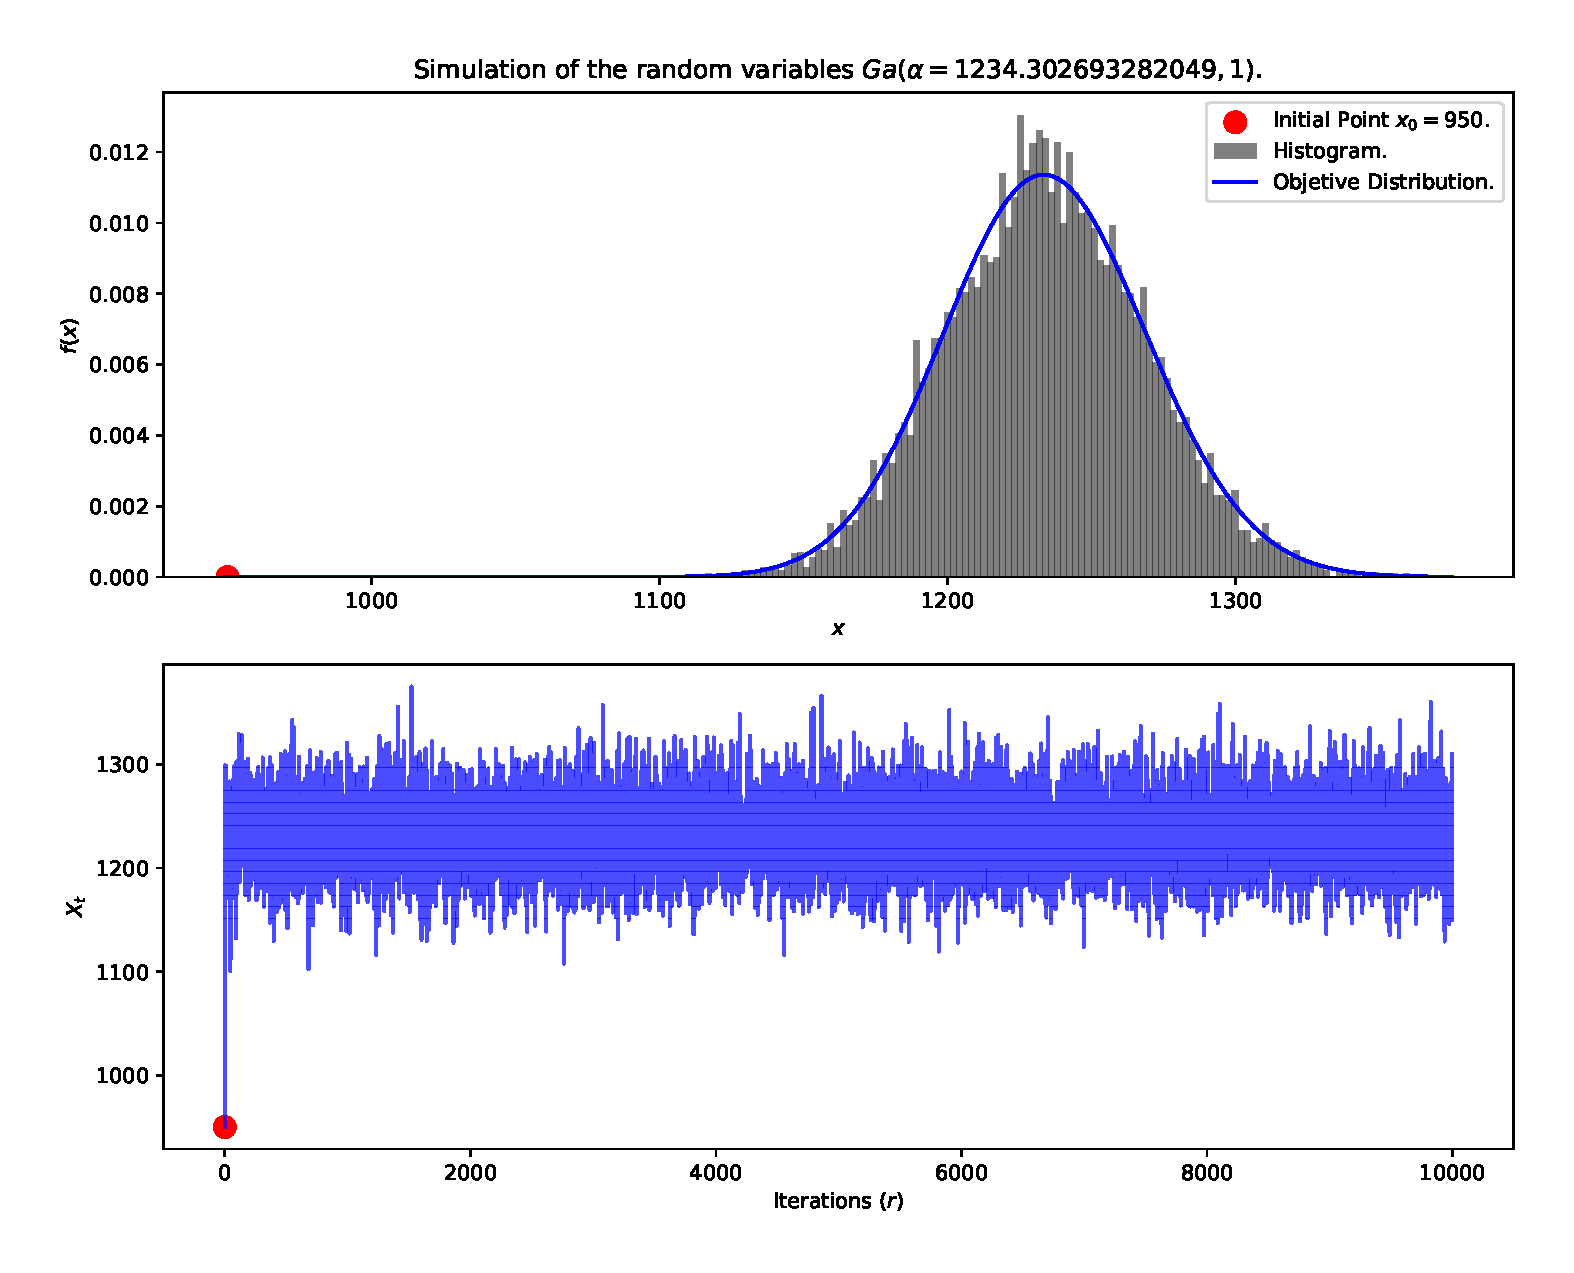
\includegraphics[width=0.6\textwidth]{IMAGENES/ex2/example3_ex2.pdf}
\end{figure}

Se simularon varios ejemplos con valores de $\alpha$ más pequeños pero, al estar tan lejos del soporte, de la distribución, tiende a generar indeterminaciones al comienzo de la cadena de Markov. Un ejemplo es el siguiente para $\alpha=10$, en donde se nota que la cadena demora un poco más en llegar a la región donde se concentra el soporte de $Gamma(10,1)$:
\begin{figure}[h!]
	\centering
	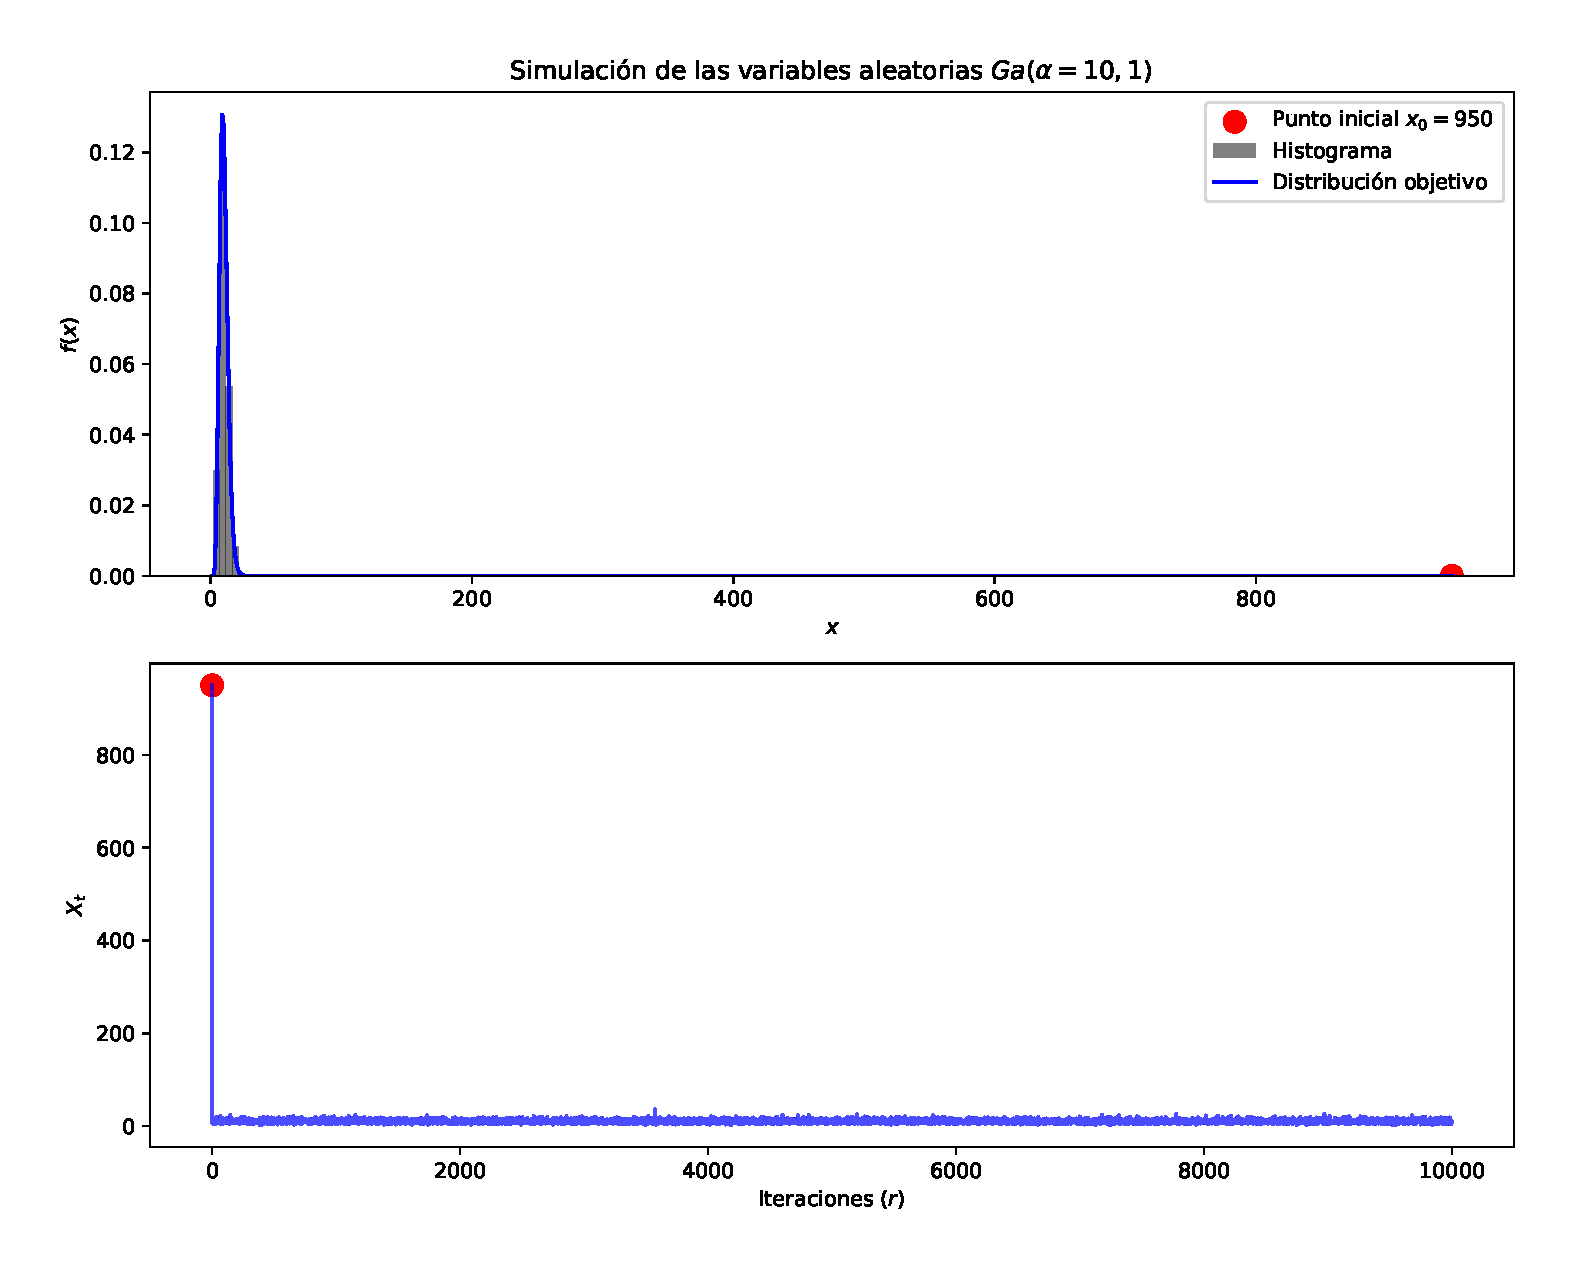
\includegraphics[width=0.8\textwidth]{IMAGENES/ejer2_alphamalo.pdf}
\end{figure}
% ------------------------------------------------------------------------------------
\newpage
.
\newpage

{\color{lightgray} \hrule}
\begin{enumerate} \setcounter{enumi}{2}
	\item Implementar Random Walk Metropolis Hasting (RWMH) donde la distribución objetivo es $\mathcal{N}_2 (\mu, \Sigma)$, con
	\begin{equation} \label{eq:7}
		\mu = \binom{3}{5}, \quad \Sigma = \left(
		\begin{array}{cc}
			1 & 0.9 \\
			0.9 & 1
		\end{array} \right).
	\end{equation}
	Utilizar como propuesta $\varepsilon_t \sim \mathcal{N}_2 (0,\sigma I)$. ¿Cómo elegir $\sigma$ para que la cadena sea eficiente? ¿Qué consecuencias tiene la elección de $\sigma$?
	
	Como experimento, elige como punto inicial $x_0 = \binom{1000}{1}$ y comenta los resultados.
\end{enumerate}

Para todos los incisos del ejercicio anterior:
\begin{itemize}
	\item Establece cual es tu distribución inicial.
	\item Grafica la evolución de la cadena.
	\item Indica cuál es el Burn-in.
	\item Comenta qué tan eficiente es la cadena.
	\item Implementa el algoritmo MH considerando una propuesta diferente.
\end{itemize}

\textcolor{BrickRed}{\it Respuesta:}

En el archivo \textcolor{mediumblue}{ejercicio3\_tarea7.py} se implementan las funciones

\begin{itemize}
	\item \textit{contornos()}: grafica los contornos de la densidad (se muestran los contornos de la distribución real debajo y se sobrepone la cadena generada.
	\item \textit{marginal\_histograms()}: genera los histogramas de las cadenas marginales.
	\item \textit{plot\_evolution\_burn\_in()}: grafica la evolución de las cadenas de Markov marginales y sobrepone el burn-in calculado.
	\item \textit{moving\_average()}: calcula la media móvil.
	\item \textit{estimate\_burn\_in()}: Determinar cuándo se estabiliza la media móvil. Esta técnica consiste en observar la media móvil de las muestras y encontrar cuándo esta se estabiliza. Es una aproximación para el burn-in.
\end{itemize}

Luego, se define la función \textit{RANDOM\_WALK\_METROPOLIS\_HASTINGS()} la cual implementa algoritmo Random Walk Metropolis-Hastings en $\mathbb{R}^n$. Toma como argumentos:
\begin{itemize}
	\item La función objetivo $f$ (en este caso es \eqref{eq:7}).
	\item El valor inicial $x_0$.
	\item La matriz de covarianza (en este caso es $\sigma I$).
	\item El número de iteraciones del algoritmo (casi siempre se usa $N = 10,000$).
\end{itemize}

Regresa la cadena de Markov simulada en $\mathbb{R}^n$ y usa el criterio de aceptación: si $y_t$ es la propuesta dada por $y_t = x_t + \varepsilon_t$ en $x_t$, entonces se acepta $y_t$ con probabilidad $\rho(x_t, y_t)$ con
\begin{equation}
	\rho(x,y) = \min\left\{1, \frac{f(y)}{f(x)} \right\}
\end{equation}
y se rechaza con probabilidad $1-\rho(x_t, y_t)$. Luego, se define la función \textit{f\_pdf()} la cual implementa \eqref{eq:7}.

Finalmente, se simulan $4$ cadenas de Markov en $\mathbb{R}^2$ con diferentes puntos iniciales y matrices de covarianza para la propuesta. Se grafican los contornos de la densidad y la evolución de la cadena de Markov en $\mathbb{R}^2$, los histogramas marginales y la evolución de las cadenas de Markov
marginales con el burn-in estimado.

% --------------------------------------------------------------------------------
\textbf{Ejemplo 1:} Se usó el punto inicial $x_0=(1,1)$, y $\sigma = 1$, i.e., la matriz de covarianzas fue $I$ y se obtuvieron los siguientes resultados:

Tasa de aceptación: $31.10\%$, burn-in estimado: $133$ iteraciones, promedio de la cadena: $[2.948, 4.944]$ y covarianza de la cadena: $\binom{1.016\quad0.911}{0.911\quad1.007}$. El algoritmo fue eficiente debido a la similitud en la magitud de $\sigma$ respecto a la lejanía de $x_0$ de $(3,5)$.
\begin{figure}[h!]
	\centering
	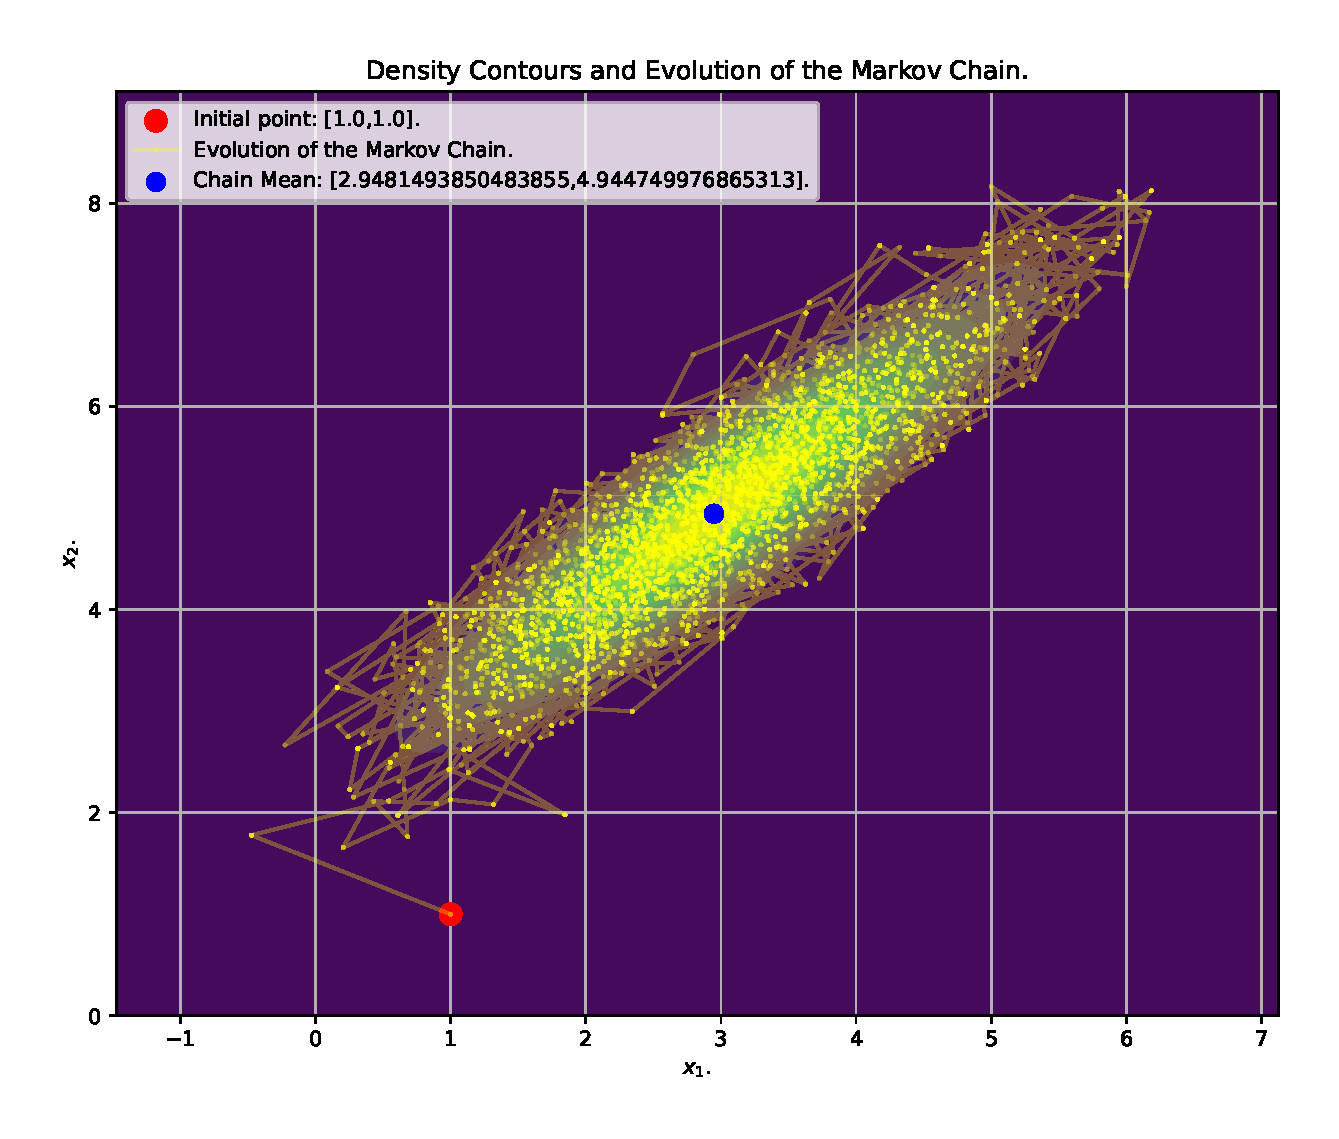
\includegraphics[width=0.84\textwidth]{IMAGENES/ex3/contour_example1.pdf}
\end{figure}
\begin{figure}[h!]
	\centering
	\begin{minipage}{0.495\textwidth}
		\centering
		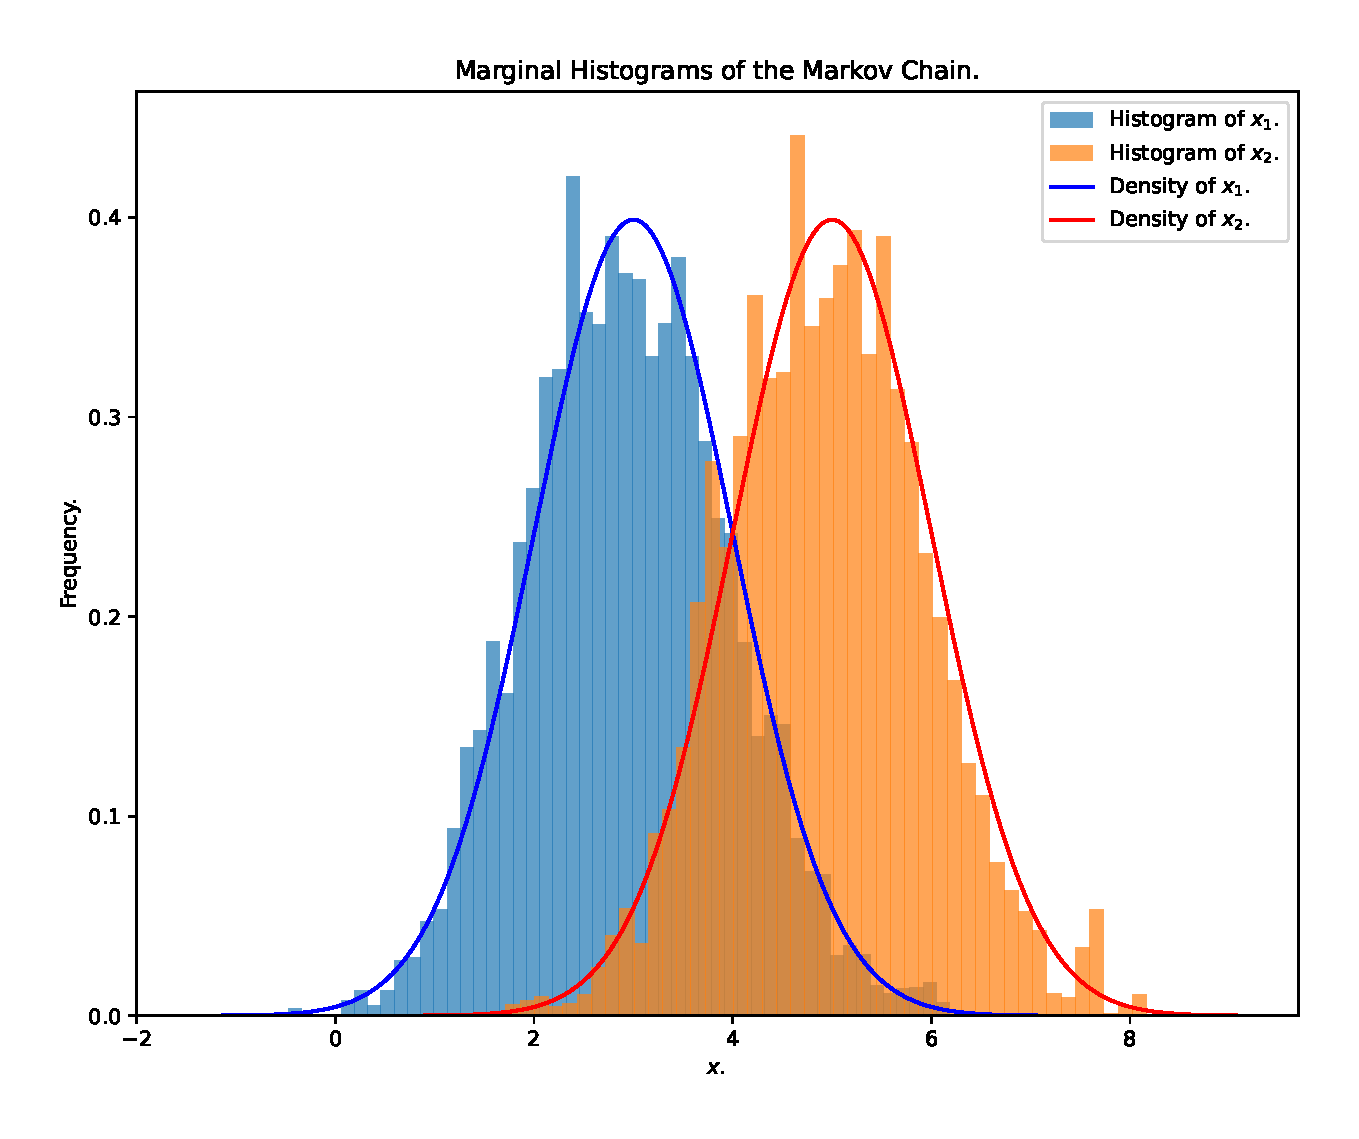
\includegraphics[width=\textwidth]{IMAGENES/ex3/histograms_example1.pdf}
	\end{minipage}
	\hfill
	\begin{minipage}{0.495\textwidth}
		\centering
		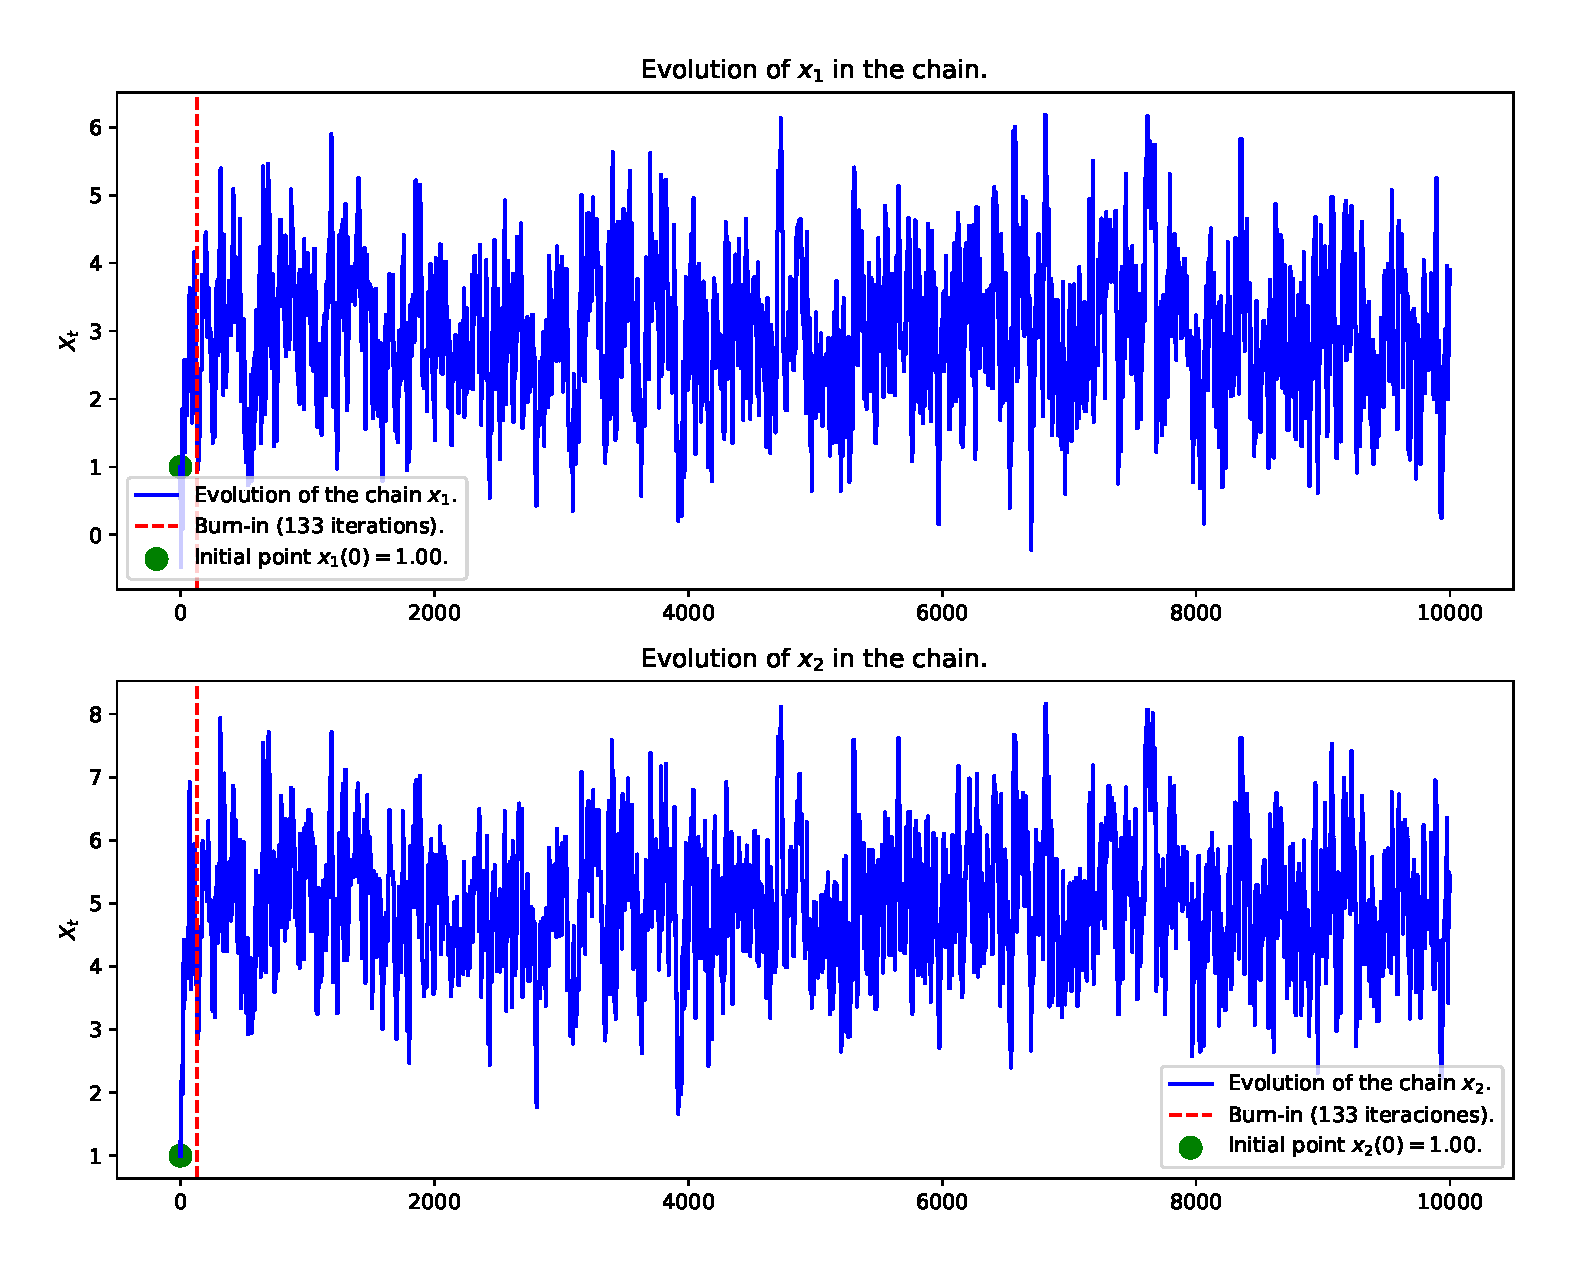
\includegraphics[width=\textwidth]{IMAGENES/ex3/evolution_example1.pdf}
	\end{minipage}
\end{figure}

% --------------------------------------------------------------------------------
\textbf{Ejemplo 2:} Se usó el punto inicial $x_0=(20,15)$, y se usó $\sigma = 20$, i.e., la matriz de covarianzas fue $20 I$ y se obtuvieron los siguientes resultados:

Tasa de aceptación: $4.06\%$, burn-in estimado: $263$ iteraciones, promedio de la cadena: $[2.931, 4.954]$ y covarianza de la cadena: $\binom{1.282\quad1.163}{1.163\quad1.266}$. El algoritmo fue eficiente debido a la similitud en la magitud de $\sigma$ respecto a la lejanía de $x_0$ de $(3,5)$.
\begin{figure}[h!]
	\centering
	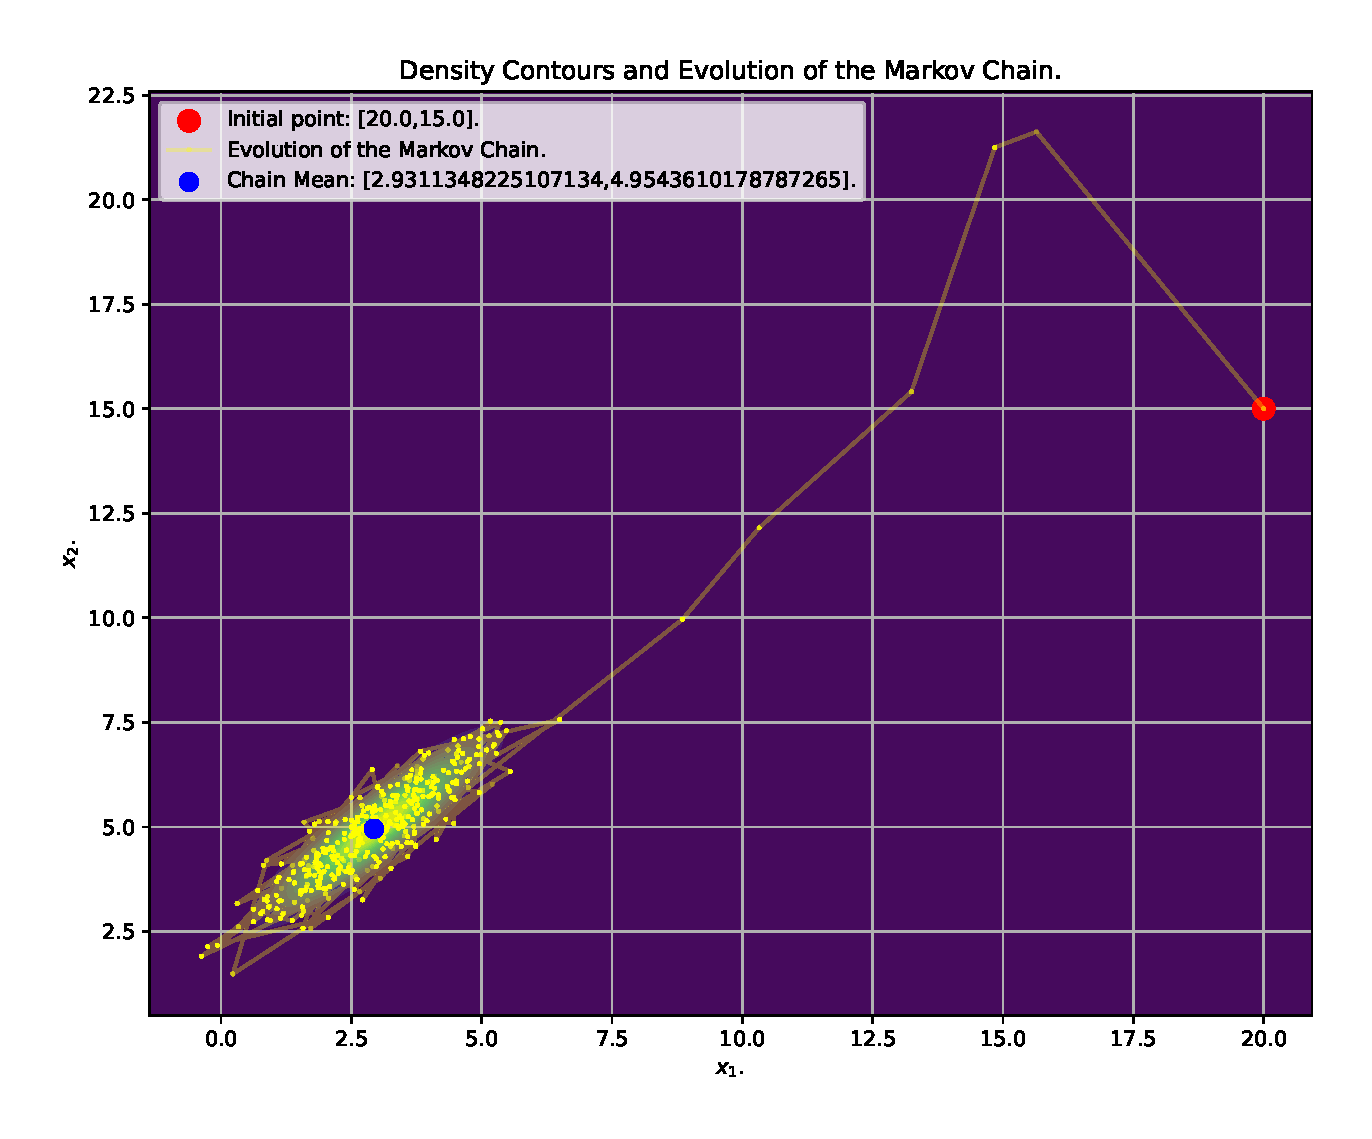
\includegraphics[width=0.87\textwidth]{IMAGENES/ex3/contour_example2.pdf}
\end{figure}
\begin{figure}[h!]
	\centering
	\begin{minipage}{0.495\textwidth}
		\centering
		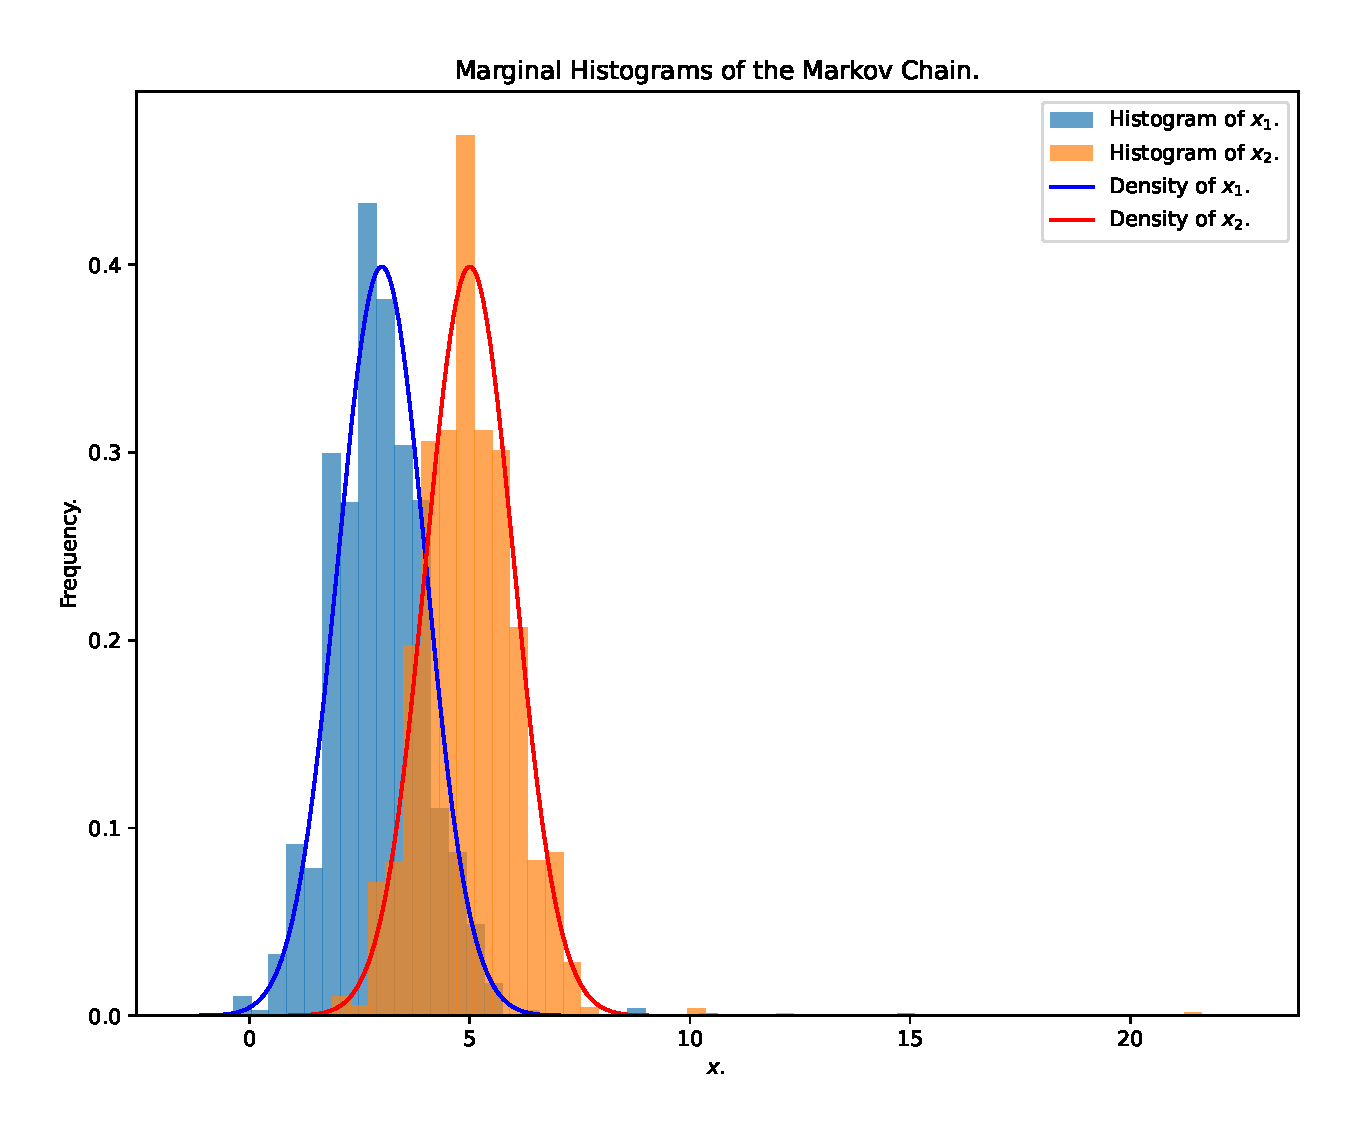
\includegraphics[width=\textwidth]{IMAGENES/ex3/histograms_example2.pdf}
	\end{minipage}
	\hfill
	\begin{minipage}{0.495\textwidth}
		\centering
		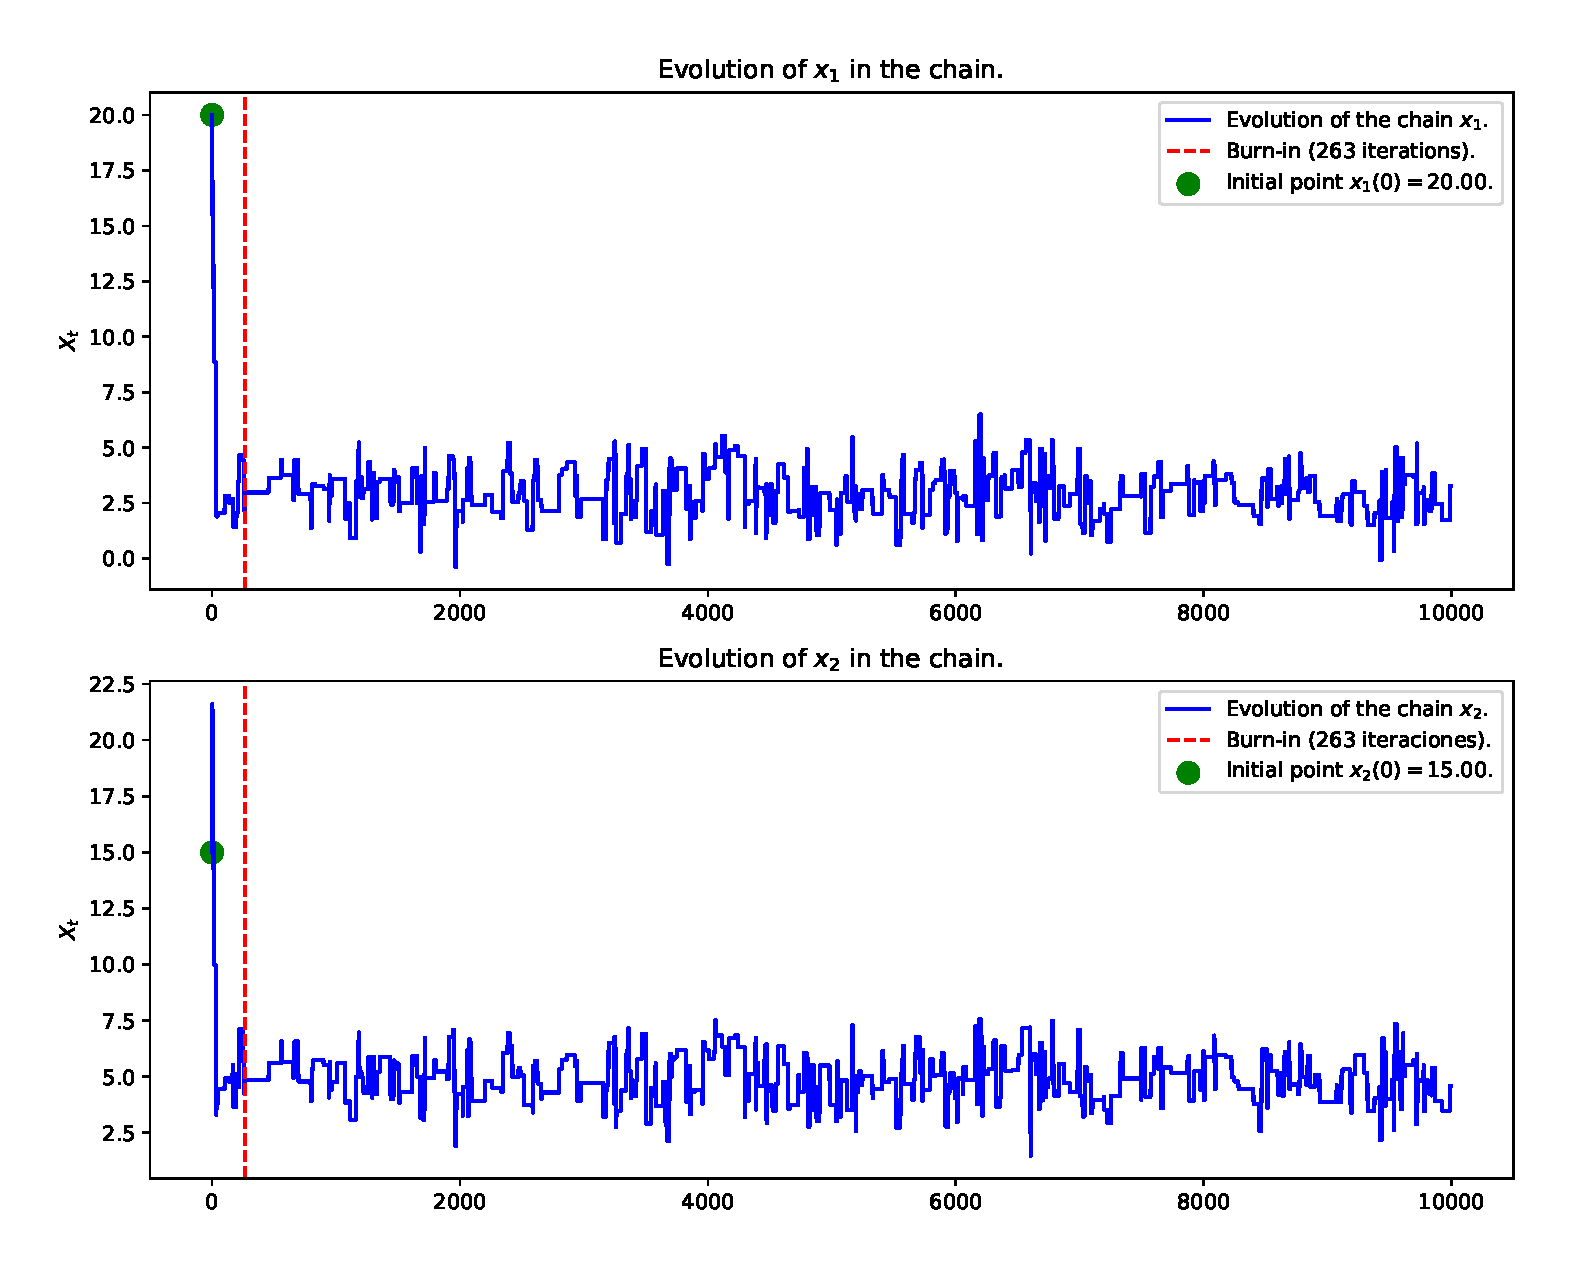
\includegraphics[width=\textwidth]{IMAGENES/ex3/evolution_example2.pdf}
	\end{minipage}
\end{figure}

% --------------------------------------------------------------------------------
\textbf{Ejemplo 3:} Se usó el punto inicial $x_0=(-20,-10)$, y se usó $\sigma = 25$, i.e., la matriz de covarianzas fue $25 I$ y se obtuvieron los siguientes resultados:

Tasa de aceptación: $4.05\%$, burn-in estimado: $162$ iteraciones, promedio de la cadena: $[2.851, 4.911]$ y covarianza de la cadena: $\binom{1.281\quad1.113}{1.113\quad1.147}$. El algoritmo fue eficiente debido a la similitud en la magitud de $\sigma$ respecto a la lejanía de $x_0$ de $(3,5)$.
\begin{figure}[h!]
	\centering
	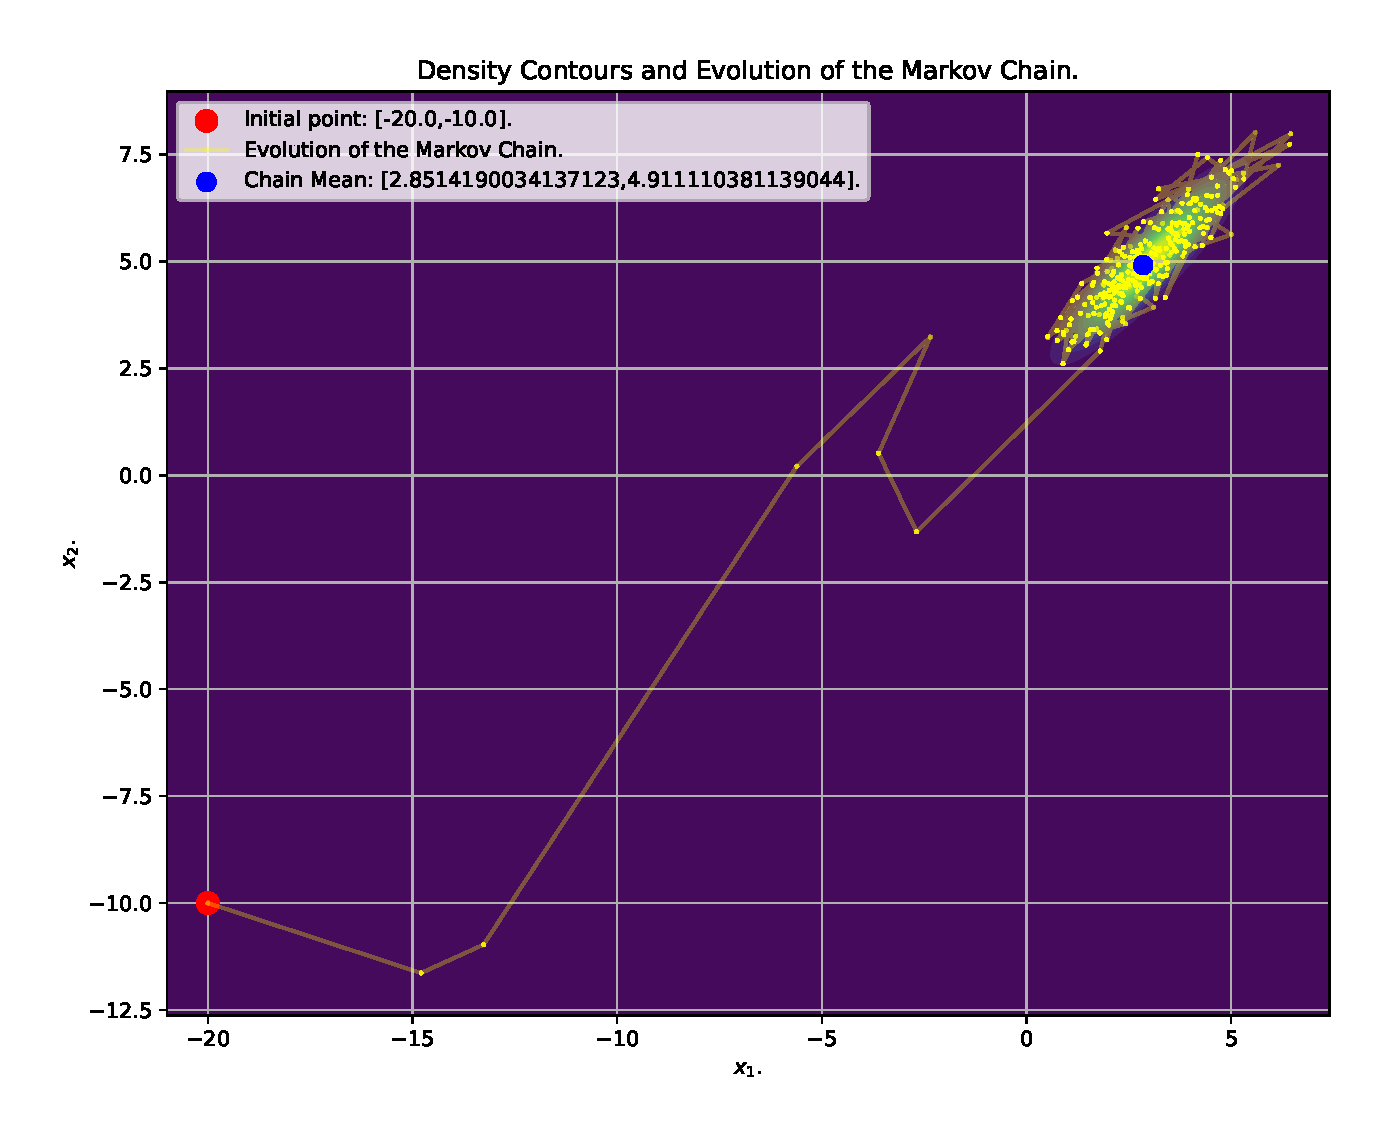
\includegraphics[width=0.87\textwidth]{IMAGENES/ex3/contour_example3.pdf}
\end{figure}
\begin{figure}[h!]
	\centering
	\begin{minipage}{0.495\textwidth}
		\centering
		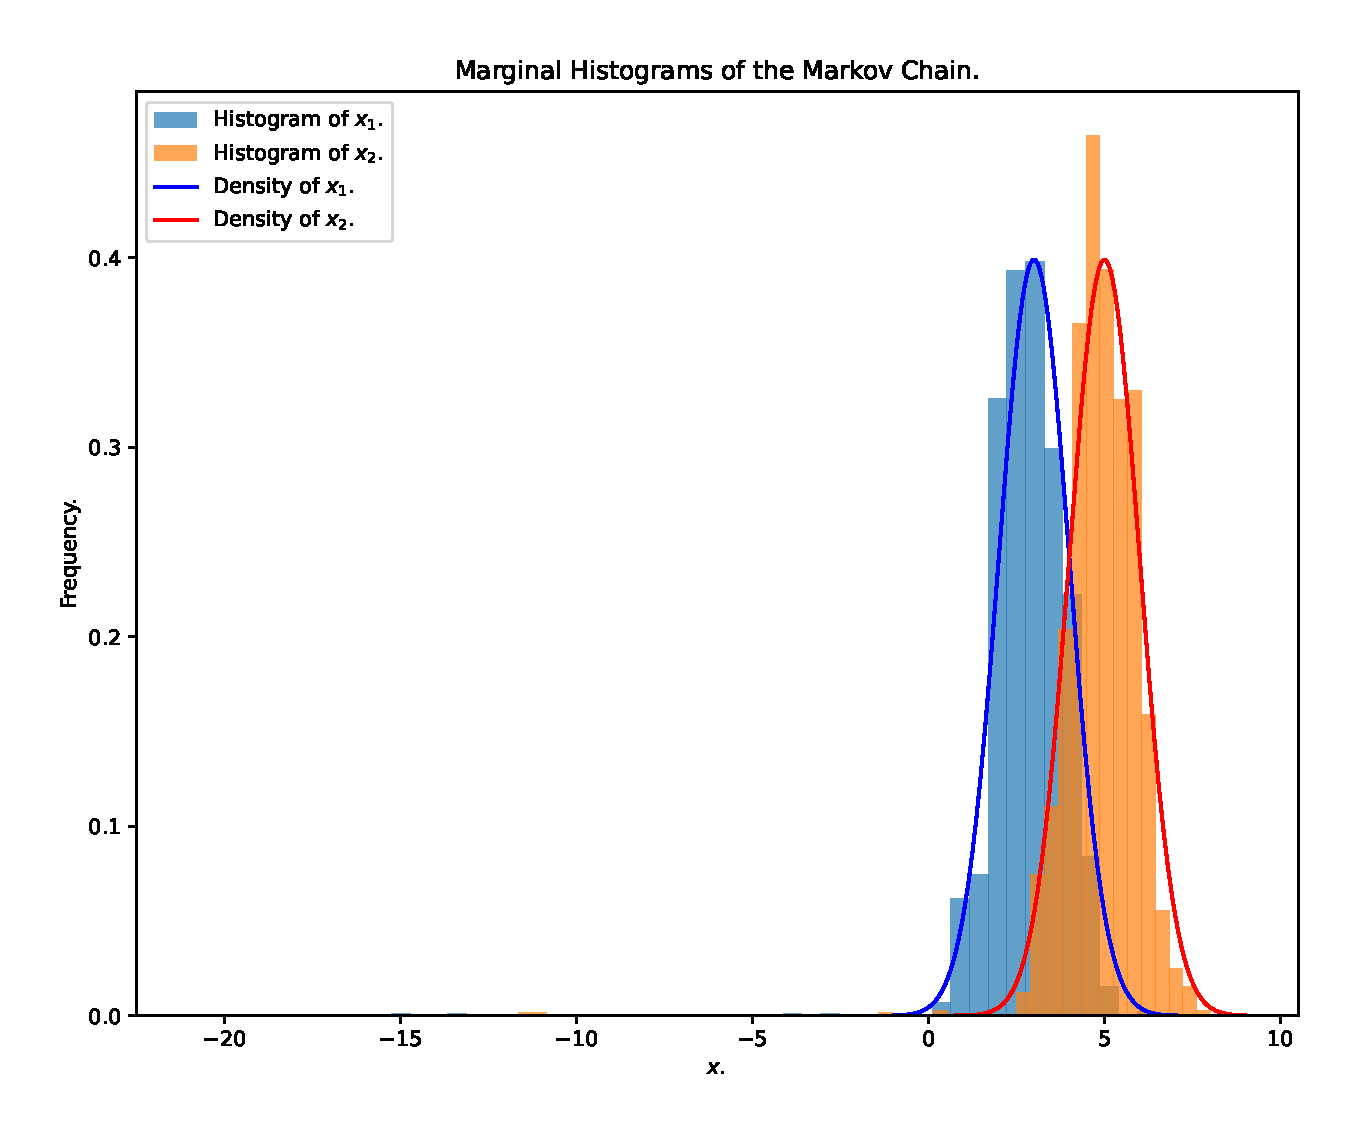
\includegraphics[width=\textwidth]{IMAGENES/ex3/histograms_example3.pdf}
	\end{minipage}
	\hfill
	\begin{minipage}{0.495\textwidth}
		\centering
		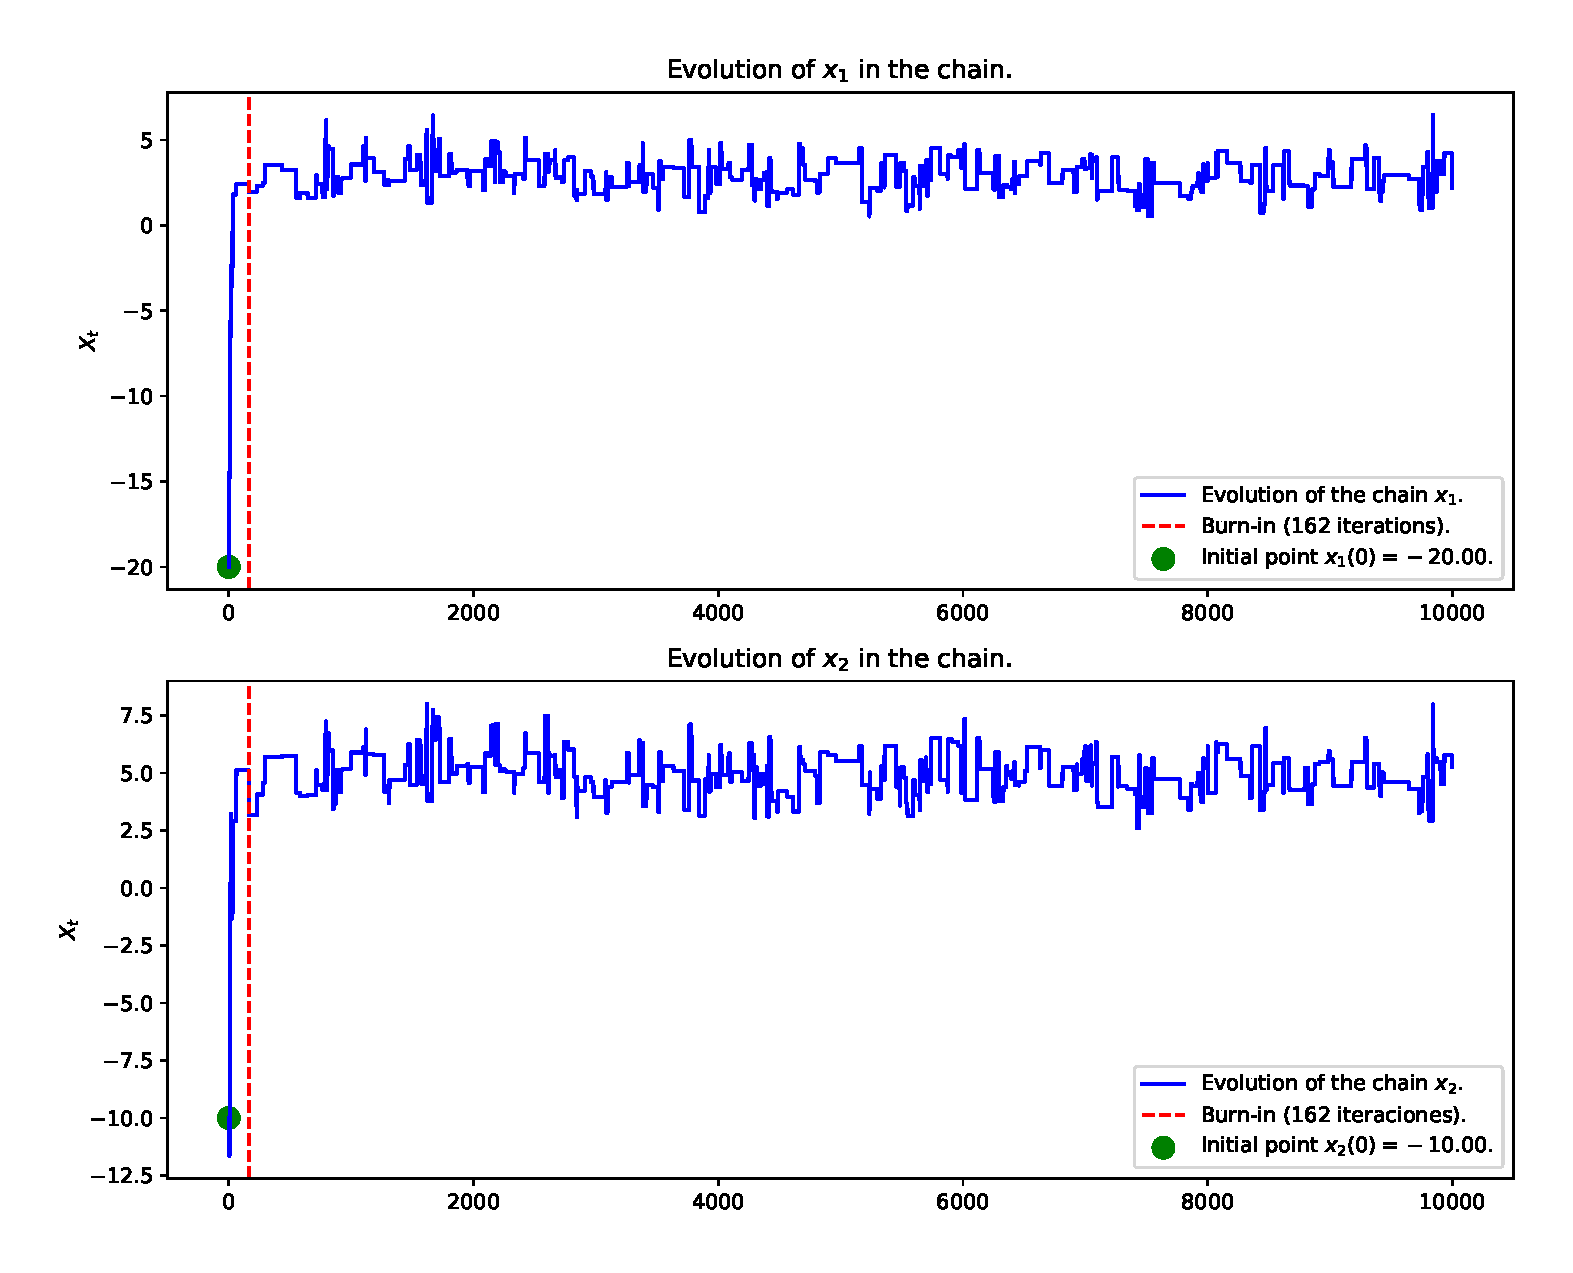
\includegraphics[width=\textwidth]{IMAGENES/ex3/evolution_example3.pdf}
	\end{minipage}
\end{figure}

% --------------------------------------------------------------------------------
\textbf{Ejemplo 4:} Se usó el punto inicial $x_0=(1000,1)$, y se usó $\sigma = 100$, i.e., la matriz de covarianzas fue $100 I$ y se obtuvieron los siguientes resultados:

Tasa de aceptación: $99.99\%$, burn-in estimado: $271$ iteraciones, promedio de la cadena: $[981.137, 1257.851]$ y covarianza de la cadena: $\binom{110724.962\quad37422.424}{37422.424\quad613530.619}$. El algoritmo no fue eficiente para ninguna configuración de parámetros debido a la lejanía de $x_0$ de $(3,5)$.
\begin{figure}[h!]
	\centering
	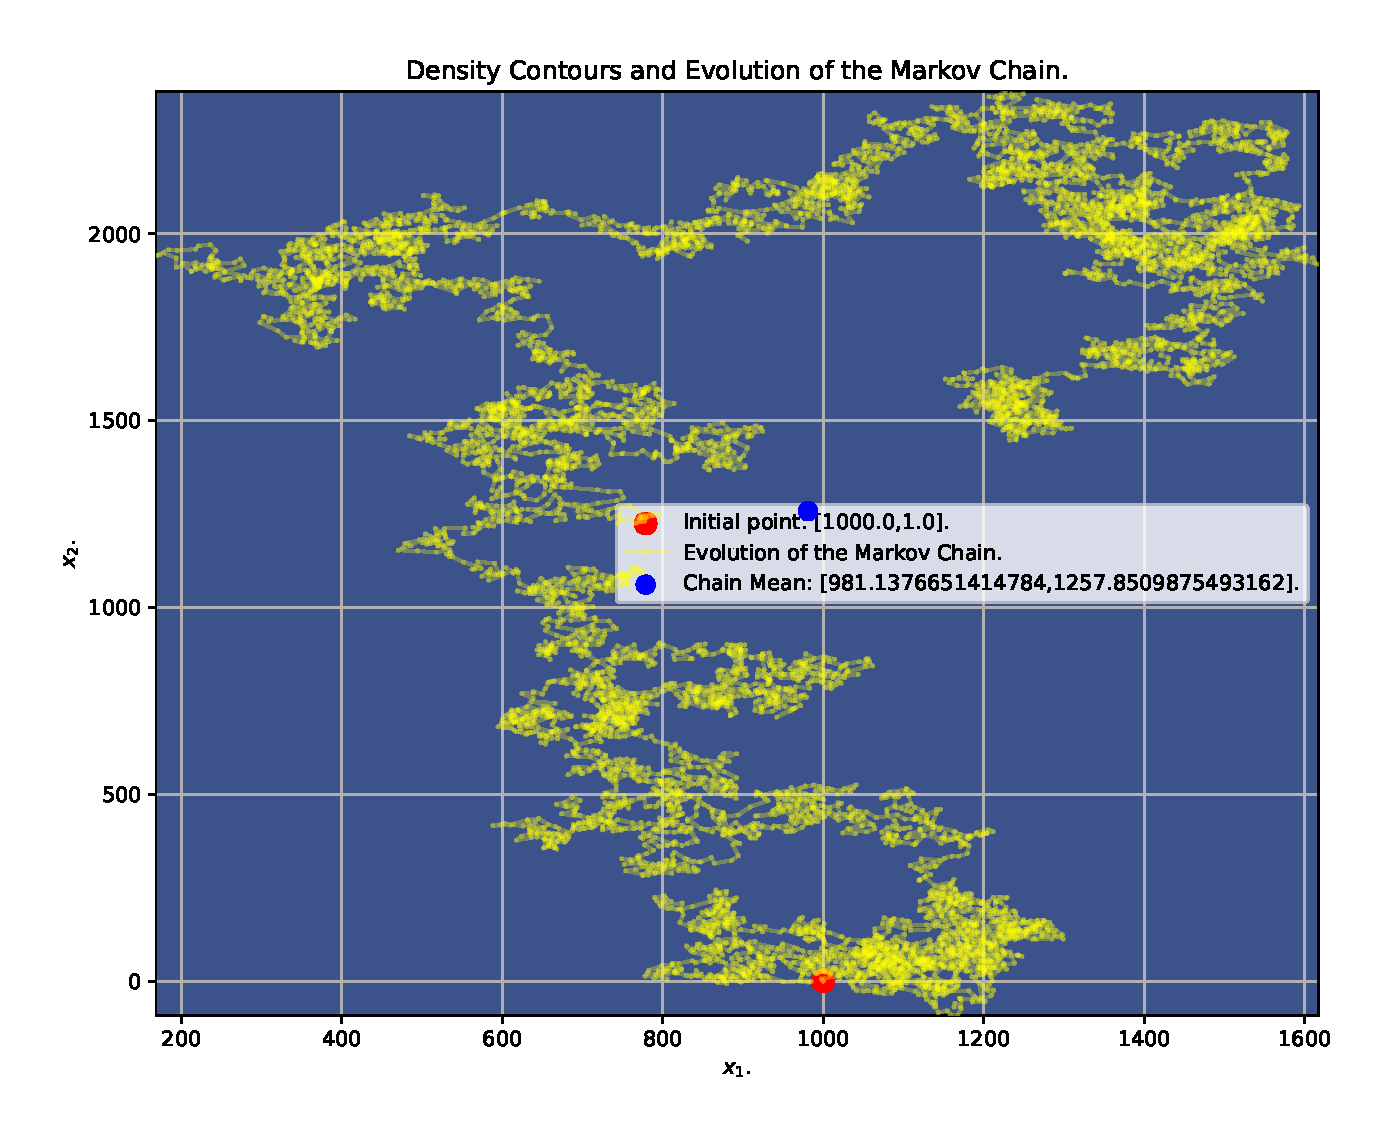
\includegraphics[width=0.87\textwidth]{IMAGENES/ex3/contour_example4.pdf}
\end{figure}

\begin{figure}[h!]
	\centering
	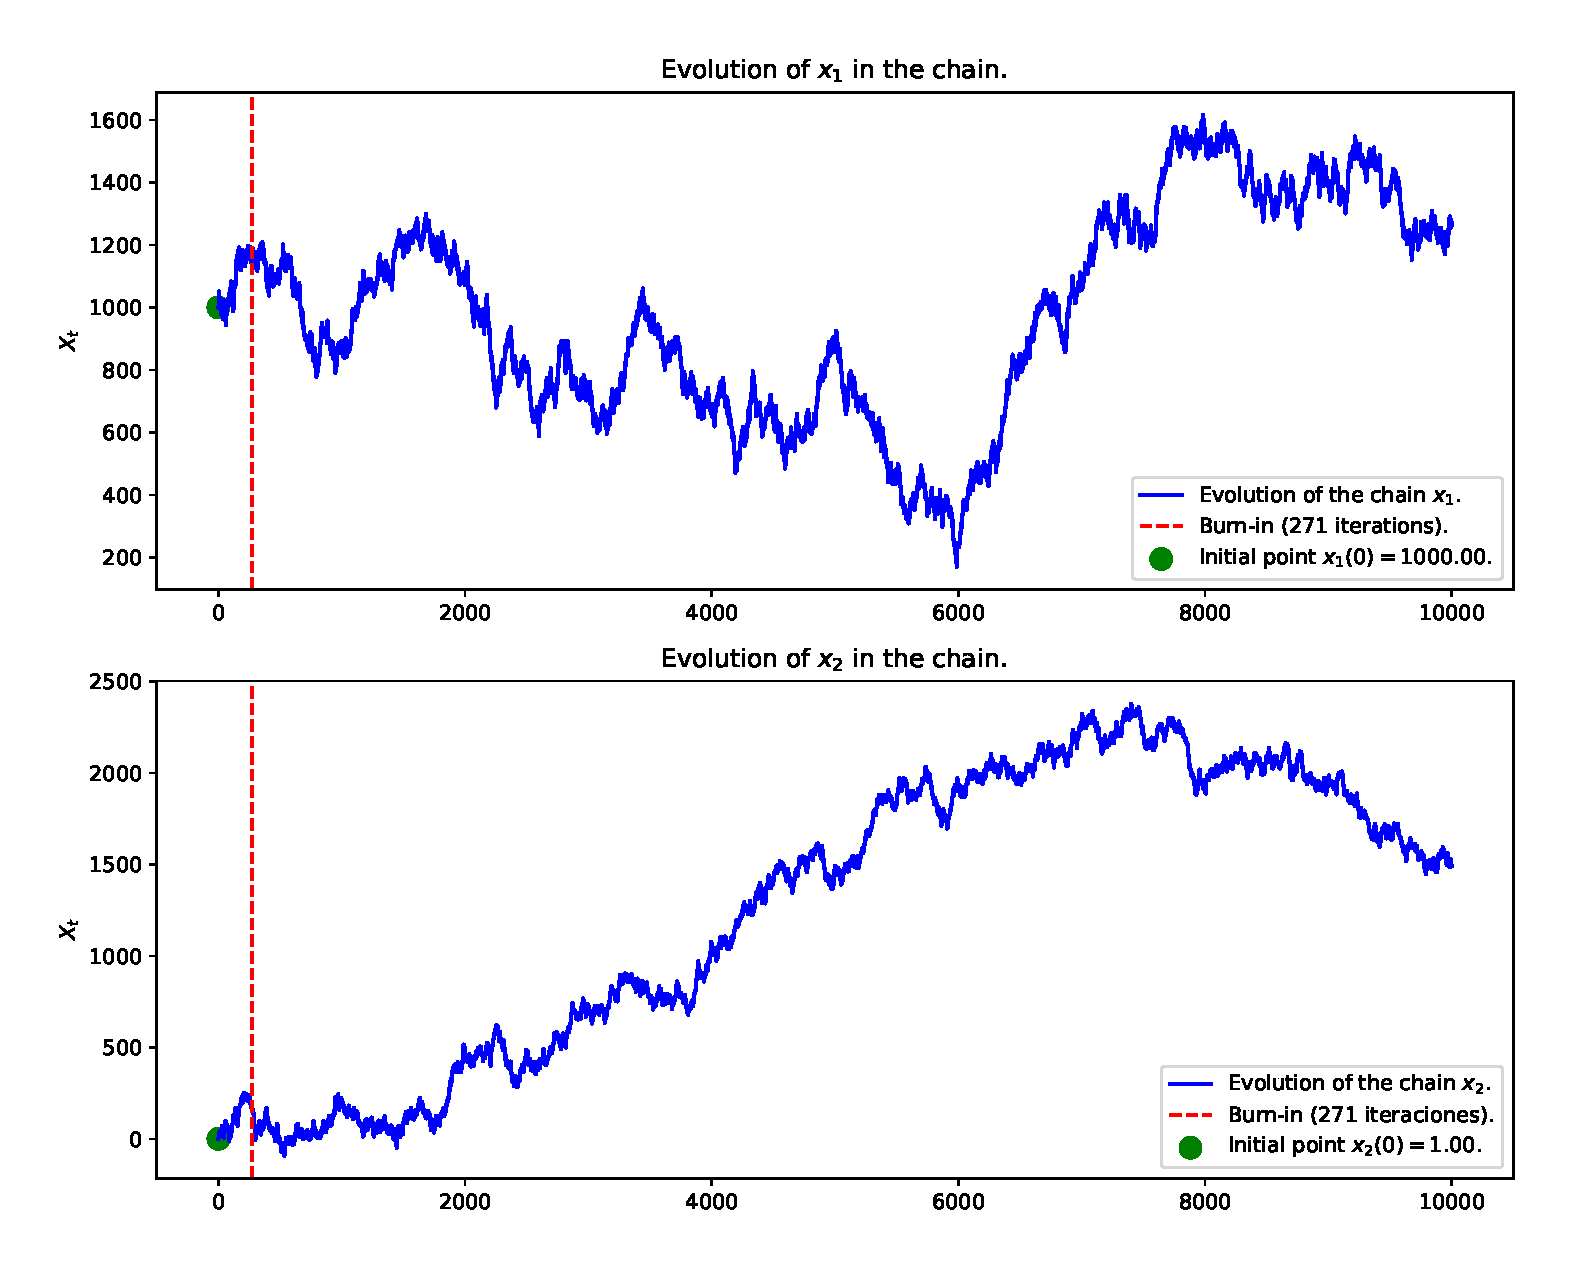
\includegraphics[width=0.8\textwidth]{IMAGENES/ex3/evolution_example4.pdf}
\end{figure}

\textbf{Comentarios finales:}

Mientras se revisaban diversos ejemplos variando parámetros como $\sigma$ y el punto inicial $x_0$, iba resultando que, según que tan lejos eligiéramos $x_0$ del punto $(3,5)$, iba a necesitar mayor varianza o un número mayor de iteraciones para que la cadena se encontrara cerca de $(3,5)$. El parámetro $\sigma$ controla el tamaño de los pasos en el proceso de Metropolis-Hastings. Se notó que las diferentes consecuencias de elegir diferentes valores de $\sigma$ son las siguientes:

\begin{itemize}
	\item $\sigma$ muy pequeño: Las propuestas estarán muy cerca del valor anterior, lo que puede resultar en una tasa de aceptación muy alta, pero la cadena se moverá muy lentamente por el espacio de estados, lo que lleva a una mayor correlación entre las muestras (un ejemplo de esto es el ejemplo $1$). En este caso, se necesitarán más iteraciones para cubrir toda la distribución objetivo, y el burn-in  será más largo.
	
	\item $\sigma$ muy grande: Las propuestas serán más lejanas, lo que puede llevar a una baja tasa de aceptación, ya que muchas propuestas serán rechazadas (ejemplos de esto son los ejemplos $2$ y $3$). La cadena puede quedarse atrapada en ciertas regiones, y será difícil explorar completamente el espacio de estados. Aquí también el burn-in puede será más largo, ya que la cadena podría tardar en estabilizarse.
\end{itemize}

Respecto a el punto inicial $x_0 = (1000,1)$ (se tiene un ejemplo en el ejemplo $4$), como se encontraba demasiado lejos de la zona donde se concentra el soporte de la distribución objetivo, generaba demasiados errores e indeterminaciones al momento de aplicar Metropolis-Hastings (específicamente al calcular la tasa de aceptación $\frac{f(y)}{f(x)}$). Los ''mejores'' resultados se tenían al usar varianzas muy grandes, sin embargo, en ninguno de los casos se logró la convergencia (no se logró la eficiencia). Esto se debe a que la probabilidad de este $x_0$ bajo la distribución objetivo es $0$, debido a su lejanía del punto $(3,5)$.



% -----------------------------------------------------------------------------------------
\vspace{5mm}
{\color{lightgray} \hrule}
\begin{enumerate} \setcounter{enumi}{3}
	\item ¿En scipy que funciones hay para simular una variable aleatoria genérica discreta? ¿tienen preproceso? [1 punto]
\end{enumerate}

\textcolor{BrickRed}{\it Respuesta:}

En SciPy, para simular una variable aleatoria discreta genérica, se puede utilizar principalmente dos funciones dentro del módulo scipy.stats: \url{https://docs.scipy.org/doc/scipy/reference/generated/scipy.stats.rv\_discrete.html}

\begin{itemize}
	\item \textit{rv\_discrete:}
\end{itemize}	
	Es una clase para definir una distribución discreta genérica. Se pueden especificar los posibles valores de la variable aleatoria y sus probabilidades asociadas.
\begin{itemize}	
	\item \textit{rv\_sample (en scipy.stats.qmc)::}
\end{itemize}
Esta es otra función útil para variables aleatorias discretas genéricas, aunque se encuentra en el submódulo qmc para \textit{muestreo cuasi-Monte Carlo}. Permite definir una distribución discreta en función de los valores y probabilidades que asignas.

Para la parte de preprocesamiento, en la documentación oficial de Scipy se menciona que antes de generar las muestras, ambas funciones verifican que:
\begin{itemize}
	\item La suma de las probabilidades sea $1$.
	\item Los valores estén correctamente definidos.
\end{itemize}

Este es el preprocesamiento que se realiza para garantizar que los datos sean válidos antes de la simulación. Además, en \textit{rv\_discrete}, las probabilidades se almacenan internamente de manera eficiente, permitiendo un acceso rápido para el muestreo durante la simulación.
% -----------------------------------------------------------------------------------------
\vspace{5mm}
{\color{lightgray} \hrule}
\begin{enumerate} \setcounter{enumi}{4}
	\item Implementar el algoritmo Adaptive Rejection Sampling y simular de una $Gamma(2,1)$ $10,000$ muestras. ¿cuando es conveniente dejar de adaptar la envolvente? [6 puntos]
\end{enumerate}

\textcolor{BrickRed}{\it Respuesta:}

Sabemos que ARS es un método de muestreo que utiliza una envolvente superior de la función objetivo para proponer muestras y luego decidir si aceptarlas o no mediante el criterio de aceptación/rechazo. Esto se implementa en el archivo  \textcolor{mediumblue}{ARS.py}.

Debido a la cantidad de código, se propone la creación de un diccionario que almacene los parámetros del método ARS y las funciones auxiliares. De esta forma, se puede acceder a los valores de los parámetros y las funciones de manera más sencilla. Además, se propone la creación de una función que inicialice los parámetros del método ARS y los guarde en el diccionario. Por último, se propone la creación de una función que genere muestras de la distribución log-concava usando el método ARS y actualice los parámetros del diccionario a medida que se generan muestras.

\textbf{Nota:} Primero se revisará, a grandes rasgos, un poco de lo visto en clase para entender mejor cada parte del código:

Sean
\begin{itemize}
	\item $f(x)$ la función proporcional a la densidad objetivo de la que se quiere muestrear.
	\item $h(x) = \log{(f(x))}$ el logaritmo de la función objetivo (es una función cóncava) con derivada $h'(x)$.
	\item $\mathcal{S}_n$ un conjunto de puntos $x_{i}$ con $i = 0,\dots n+1$ en el soporte de $f$ tales que $h(x_i) = \log{(f(x_i))}$ se conoce hasta una constante.
	\item $\mathcal{L}_{i}(x)$ la recta con pendiente $h^{'}(x_{i})$ que pasa por el punto $(x_i, h(x_i))$, es decir, la recta tangente a $h$.
\end{itemize}

Notemos que $\mathcal{L}_{i}$ siempre está por encima de $h$, esto es posible gracias a la concavidad de $h$.
\begin{figure}[h!]
	\centering
	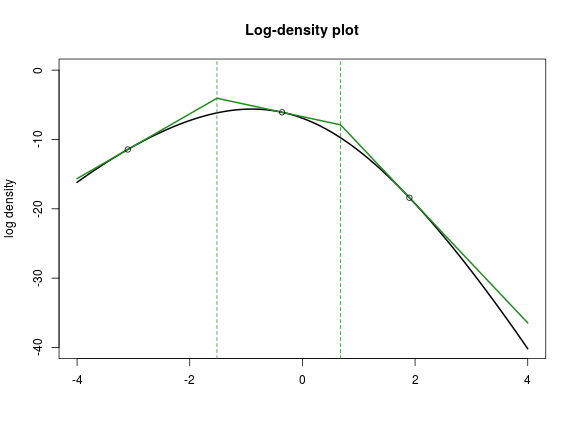
\includegraphics[width=0.65\textwidth]{IMAGENES/libro}
\end{figure}

\textbf{Intersecciones entre las $\mathcal{L}$'s}

Notemos que en cada intervalo $[x_i, x_{i+1}]$, se tiene un par de rectas tangentes correspondientes a $x_i$ y $x_{i+1}$. Además cuentan con una intersección para algún punto $z_i\in[x_i, x_{i+1}]$ (ver imágen anterior). Por la ecuación de la recta que úne dos puntos, tenemos que estas rectas están dadas por
\begin{equation}
	\mathcal{L}_{i} (x)= h(x_{i}) + h^{'}(x_{i}) (x - x_{i}) \text{ y } \mathcal{L}_{i+1} (x) =  h(x_{i+1}) + h^{'}(x_{i+1}) (x - x_{i+1})
\end{equation}
Entonces, la intersección es aquel $z_i$ tal que cumpla ambas ecuaciones anteriores. Después de igualar estas expresiones y hacer los cálculos necesarios, se tiene que:
\begin{equation}\label{eq:7}
	z_{i} = -\frac{h_{i+1} - h_{i} - \left(h_{i+1}^{'} x_{i+1} - h_{i}^{'} x_{i}\right)}{h_{i+1}^{'} - h_{i}^{'}}
\end{equation} 
donde $h_{j} = h(x_{j})$ y $h_{j}^{'} = h^{'}(x_{j})$. De esta forma, la envolvente superior está dada por:

$$	
	u(x) :=
	\begin{cases}
		h(x_0) + h^{'}(x_0)(x-x_0) = \mathcal{L}_{0} (x) & \text{si } x \leq z_0, \\
		\hspace{3cm}\vdots \\
		h(x_i) + h^{'}(x_i)(x-x_i) = \mathcal{L}_{i} (x) & \text{si } z_{i} \leq x \leq z_{i+1}, \\
		\hspace{3cm}\vdots \\
		h(x_n) + h^{'}(x_n)(x-x_n) = \mathcal{L}_{n} (x) & \text{si } z_n \leq x, \\
	\end{cases}
$$
y la envolvente en cada punto de intersección es
\begin{equation} \label{eq:8}
	u_{i} := \mathcal{L}_{i} (z_{i}).
\end{equation} 

\newpage
\textbf{Área bajo las rectas tangentes}

A continuación, se necesitan calcular los segmentos de área bajo las rectas tangentes de la envolvente superior, o bien, el área acumulada bajo las tangentes de la envolvente superior. Esto es necesario para normalizar las probabilidades durante el proceso de muestreo:

Se tiene que $u(x) = \mathcal{L}_{i} (x)$ en $[x_i, x_{i+1}]$, así
\begin{equation*}
	e^{u(x)} = e^{\mathcal{L}_{i} (x)} = e^{h(x_{i}) + h^{'}(x_{i}) (x - x_{i})} = e^{h(x_{i})} e^{h^{'}(x_{i}) (x - x_{i})}
\end{equation*}
El área bajo la curva $e^{u(x)}$ en $[x_i, x_{i+1}]$ es:
\begin{equation} \label{eq:9}
	e^{h(x_{i})} \int_{x_{i}}^{x_{i+1}}  e^{h^{'}(x_{i}) (x - x_{i})} dx = e^{h(x_{i})} \frac{e^{h^{'}(x_{i}) (x_{i+1} - x_{i})} - 1}{h^{'}(x_{i})} = \frac{e^{u(x_{i+1})} - e^{u(x_{i})}}{h^{'}(x_{i})},
\end{equation}
ya que $u(x_{i+1}) = h(x_{i}) + h^{'}(x_{i}) (x_{i+1} - x_{i})$. Entonces, la suma acumulada de estos términos es:
\begin{equation}\label{eq:10}
	s_{j} := \sum_{i=1}^{j}  \frac{e^{u(x_{i+1})} - e^{u(x_{i})}}{h^{'}(x_{i})}.
\end{equation}
Y la última suma acumulativa es: 
\begin{equation} \label{eq:11}
	cu_i := s_{n}.
\end{equation}

\vspace{5mm}
\begin{center}
	\textcolor{mediumblue}{----------- ARS.py -----------}
\end{center}

A continuación, se da una descipción detallada de lo que hacen las funciones implementadas en el archivo:

\begin{itemize}
\item Las expresiones \eqref{eq:7}, \eqref{eq:8}, \eqref{eq:10}, \eqref{eq:11} se calculan con la función auxiliar \textit{intersecciones\_y\_areas()}, la cual nos ayuda a hacer estos cálculos para una muestra dada de $x_i$, sus evaluaciones $h(x_i)$ y sus pendientes $h^{'}(x_i)$. 

\item Posteriormente, se da la función \textit{DIC\_INICIAL()} la cual crea un diccionario con los parámetros iniciales para el método de muestreo de Adaptive Rejection Sampling (ARS).
Inicializa los puntos $x_i$, los valores $h(x_i)$, sus pendientes $h^{'}(x_i)$ y usa la función \textit{intersecciones\_y\_areas()} para calcular los puntos de intersección $z_i$ de las tangentes. Además, calcula la envolvente superior $u(x) = h(x_i) + h^{'}(x_i) (x - x_i)$ y el área acumulada $s_i$ bajo las tangentes. El área acumulada hasta el último punto se guarda en $cu_i$. Esta función regresa el diccionario de parámetros inicializados.

\item Después, se tiene la función \textit{muestreo()} la cual devuelve un solo valor muestreado aleatoriamente desde la envolvente superior de la función log-concava que está siendo muestreada y el índice del segmento en el que cayó el valor muestreado. Genera un número aleatorio $u\sim\mathcal{U}(0,1)$ y este se utiliza para seleccionar un punto en la envolvente superior, basándose en las áreas acumuladas bajo las rectas tangentes que representan la envolvente superior ya que se quiere encontrar en qué segmento de la envolvente superior se encuentra el valor de $u$:
\begin{equation} \label{eq:12}
	i = \max \left\{ j \mid \frac{s_j}{cu_{i}} < u \right\}
\end{equation}
La función usa el concepto de muestreo inverso por transformada. Al generar un número aleatorio  $u$, se busca un punto cuya área acumulada (normalizada) hasta dicho punto sea igual a $u$ (como el ejemplo contructivo visto en clase). Una vez identificado el segmento adecuado, se muestrea un punto dentro de ese segmento usando las propiedades locales de la función log-convexa (como las pendientes y las alturas).

Una vez encontrado el segmento $i$, se calcula el punto  $x_t$  dentro de ese segmento de la envolvente superior. Para esto, se usa la fórmula:
\begin{equation} \label{eq:13}
	x_t = x_i + \frac{-h(x_i) + \log \left( h^{'}(x_i) \cdot \left( cu_i \cdot u - s_i \right) + e^{u_i} \right)}{h^{'}(x_i)}
\end{equation}
Esta se obtuvo gracias a que, ya habíamos visto que para $x_t\in[x_{i}, x_{i+1}]$, entonces
\begin{equation*}
	\int_{x_{i}}^{x_t} e^{u(x)} dx =  \frac{e^{u(x_t)} - e^{u(x_{i})}}{h^{'}(x_{i})}
\end{equation*}
y se quiere que esta área acumulada se corresponda con el número aleatorio $u$ generado en $[0, 1]$, es decir, se necesita resolver la ecuación:
\begin{equation*}
	\frac{e^{u(x_t)} - e^{u(x_{i})}}{h^{'}(x_{i})} = cu_i \cdot u - s_i.
\end{equation*}
Resolviendo esta ecuación para $x_t$, de obtiene le expresión \eqref{eq:13}.

\item En la función \textit{insertar\_puntos()} se actualizan las envolventes con nuevos puntos. Si no se proporcionan, solo recalcula la envolvente a partir de los puntos existentes. Si se proporcionan nuevos puntos, se concatenan con los existentes y se recalcula la envolvente. Además, se recalculan los puntos de intersección de las tangentes y el área acumulada bajo la
envolvente con ayuda de la función auxiliar \textit{intersecciones\_y\_areas()}.

\item Finalmente, se tiene la función \textit{aceptacion\_rechazo()}. La cual genera $N$  muestras a partir de la envolvente superior y actualizarla si es necesario. Esta función implementa el muestreo adaptativo, aprovechando el método ARS. La lógica se basa en aceptar o rechazar muestras propuestas de acuerdo con la envolvente superior y la función subyacente. Usa a la función \textit{muestreo()} para obtener una propuesta de muestra  $x_t$  y el índice del segmento de la envolvente superior donde está situada. Calcular la altura de la envolvente superior en  $x_t$, luego, genera un número aleatorio $u\sim\mathcal{U}$ para decidir si se acepta $x_t$ o no. Esto se logra comparando a $u$ con la probabilidad de aceptación:
\begin{equation} \label{eq:14}
	\exp{\left(h(x_t)-u(x_t)\right)}
\end{equation}
(Esto se deriva de la relación entre la envolvente superior y la función objetivo). Si
\begin{equation} \label{eq:15}
	u <	\exp{\left(h(x_t)-u(x_t)\right)}
\end{equation}
se acepta la muestra y se almacena y se actualiza $\mathcal{S}_n$.
\end{itemize}

\textbf{Ejemplos de uso:}
	
Al final del archivo \textcolor{mediumblue}{ARS.py} se tiene un par de ejemplos:
\begin{itemize}
	\item Generación de una distribución normal $X\sim\mathcal{N}(2,3)$. Para esto, necesitamos $h$ cóncava tal que $e^{h}$ sea proporcional a la distribución de $X$. Para esto, se propone una alteración de la distribución Log Normal:
	\begin{equation}
		h(x,\mu,\sigma) = -\frac{(x-\mu)^2}{2\sigma^{2}}
	\end{equation}
	con derivada:
	\begin{equation}
		h^{'}(x, \mu, \sigma) = -\frac{(x-\mu)}{\sigma^2}
	\end{equation}
	Notemos que $e^{h(x)} \propto \mathcal{N}(\mu,\sigma)$. Se obtuvo el siguiente resultado y se comparó con la distribución verdadera $X\sim\mathcal{N}(2,3)$:
	
	\begin{figure}[h!]
		\centering
		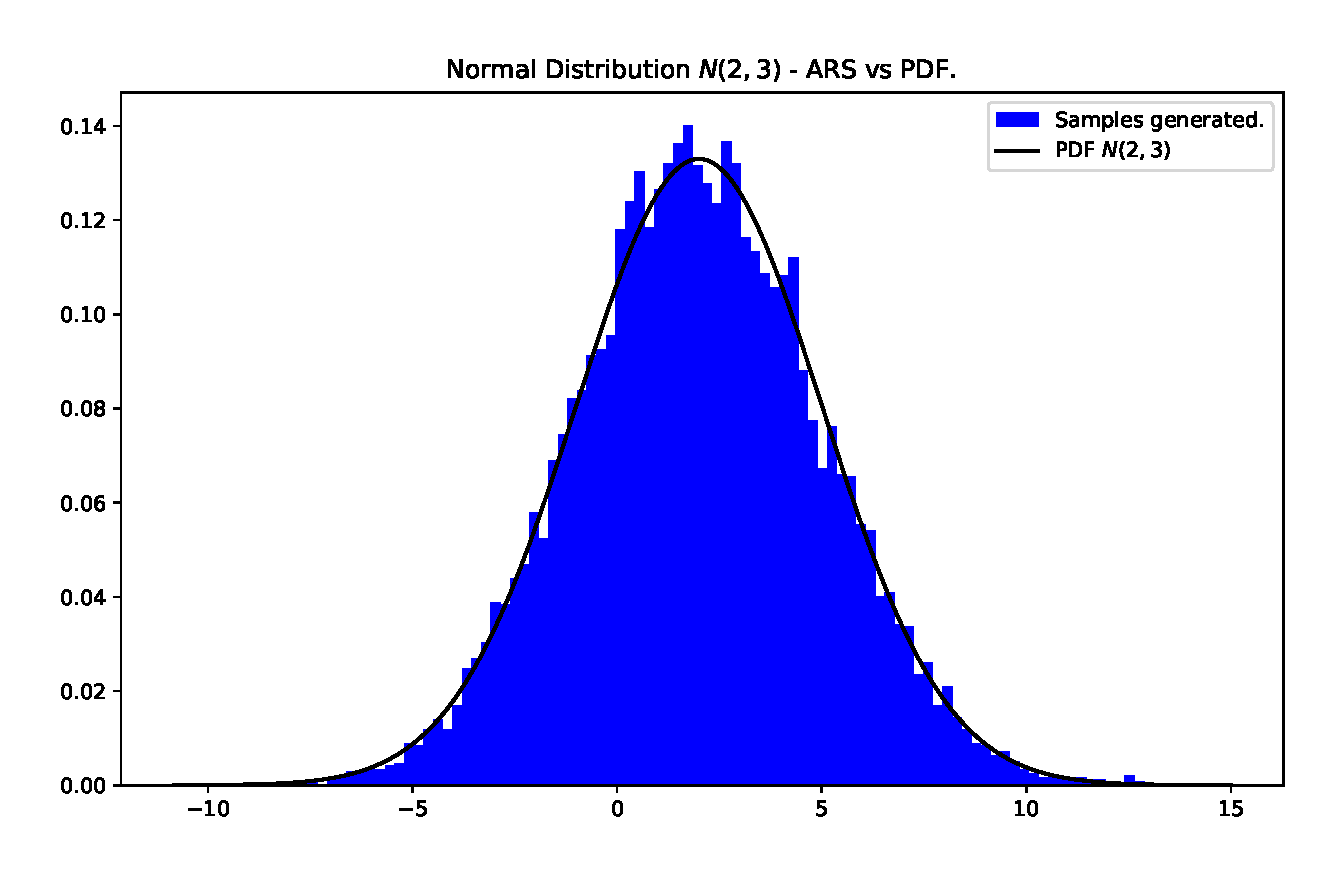
\includegraphics[width=0.59\textwidth]{IMAGENES/ARS_example1.pdf}
	\end{figure}
	
	\item De la misma forma, se generó una distribución $Beta(1.3,2.7)$:
	\begin{figure}[h!]
		\centering
		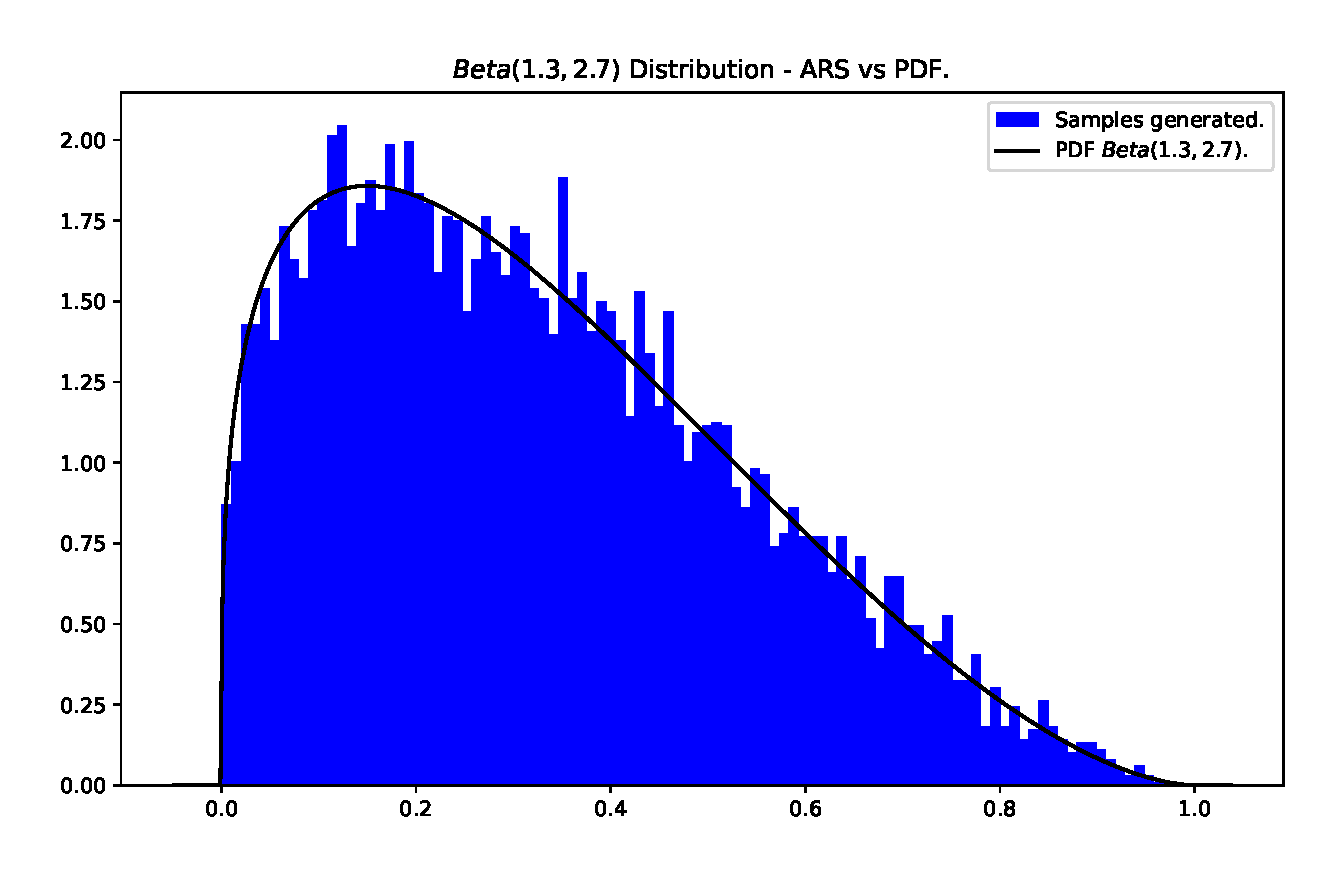
\includegraphics[width=0.59\textwidth]{IMAGENES/ARS_example2.pdf}
	\end{figure}
\end{itemize}

\textbf{Distribución $Gamma(2,1)$}

Para generar esta distribución, en el archivo \textcolor{mediumblue}{ejercicio5\_tarea5.py}, se propone el uso de
\begin{equation}
	h(x,k, \theta) = (k-1)\log{x} - \frac{x}{\theta}
\end{equation}
con derivada:
\begin{equation}
	h^{'}(x,k,\theta) = \frac{k-1}{x} - \frac{1}{\theta}
\end{equation}
En la cual podemos notar que
\begin{equation}
		e^{h(x)} = e^{(k-1)\log{x} - \frac{x}{\theta}} = x^{k-1} e^{-\frac{x}{\theta}} \propto \frac{1}{\Gamma(k) \theta^{k}} x^{k-1} e^{-\frac{x}{\theta}}
\end{equation}
que es la distribución de $X\sim Gamma(k,\theta)$. Esto se usa en \textcolor{mediumblue}{ejercicio5\_tarea5.py} para generar $N=10000$ muestras de $Gamma(2,1)$, para los puntos iniciales: $\mathcal{S} = \{0.1,0.5,2,5,10\}$ en el soporte de $X$. Esto nos genera:

\begin{figure}[h!]
	\centering
	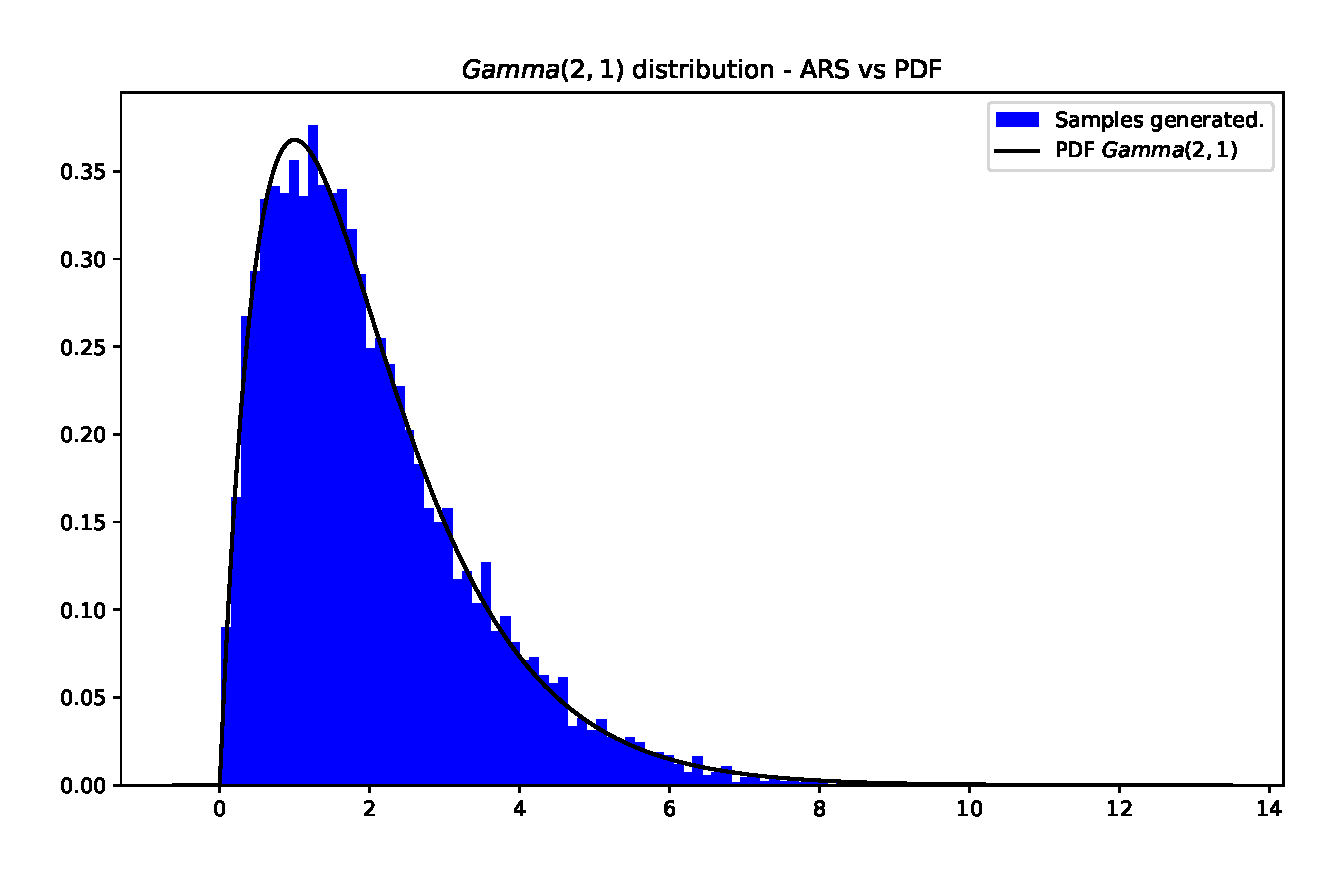
\includegraphics[width=0.59\textwidth]{IMAGENES/ARS_gamma.pdf}
\end{figure}

Para responder la pregunta ¿cuándo es conveniente dejar de adaptar la envolvente?:

En ARS, inicialmente se utilizan algunos puntos para definir la envolvente superior (compuesta por segmentos lineales), pero después, cada vez que se rechaza un valor propuesto o cuando se detecta que la envolvente puede mejorar, se añaden nuevos puntos de tangencia.

Si el criterio de rechazo se cumple en una proporción suficientemente baja (es decir, la mayoría de las muestras propuestas son aceptadas), significa que la envolvente ya está ajustada de manera adecuada. En este caso, puedes dejar de adaptar la envolvente porque el proceso de muestreo es eficiente. O bien, fijar un límite máximo para el número de puntos para mejorar el costo computacional. En mi implementación se usó un número máximo de $100$ puntos.

\end{document}
